% Options for packages loaded elsewhere
\PassOptionsToPackage{unicode}{hyperref}
\PassOptionsToPackage{hyphens}{url}
%
\documentclass[
]{book}
\usepackage{lmodern}
\usepackage{amssymb,amsmath}
\usepackage{ifxetex,ifluatex}
\ifnum 0\ifxetex 1\fi\ifluatex 1\fi=0 % if pdftex
  \usepackage[T1]{fontenc}
  \usepackage[utf8]{inputenc}
  \usepackage{textcomp} % provide euro and other symbols
\else % if luatex or xetex
  \usepackage{unicode-math}
  \defaultfontfeatures{Scale=MatchLowercase}
  \defaultfontfeatures[\rmfamily]{Ligatures=TeX,Scale=1}
\fi
% Use upquote if available, for straight quotes in verbatim environments
\IfFileExists{upquote.sty}{\usepackage{upquote}}{}
\IfFileExists{microtype.sty}{% use microtype if available
  \usepackage[]{microtype}
  \UseMicrotypeSet[protrusion]{basicmath} % disable protrusion for tt fonts
}{}
\makeatletter
\@ifundefined{KOMAClassName}{% if non-KOMA class
  \IfFileExists{parskip.sty}{%
    \usepackage{parskip}
  }{% else
    \setlength{\parindent}{0pt}
    \setlength{\parskip}{6pt plus 2pt minus 1pt}}
}{% if KOMA class
  \KOMAoptions{parskip=half}}
\makeatother
\usepackage{xcolor}
\IfFileExists{xurl.sty}{\usepackage{xurl}}{} % add URL line breaks if available
\IfFileExists{bookmark.sty}{\usepackage{bookmark}}{\usepackage{hyperref}}
\hypersetup{
  pdftitle={Boletín Estadístico Sede Tumaco},
  pdfauthor={ Universidad Nacional de Colombia   Sede Tumaco},
  hidelinks,
  pdfcreator={LaTeX via pandoc}}
\urlstyle{same} % disable monospaced font for URLs
\usepackage{longtable,booktabs}
% Correct order of tables after \paragraph or \subparagraph
\usepackage{etoolbox}
\makeatletter
\patchcmd\longtable{\par}{\if@noskipsec\mbox{}\fi\par}{}{}
\makeatother
% Allow footnotes in longtable head/foot
\IfFileExists{footnotehyper.sty}{\usepackage{footnotehyper}}{\usepackage{footnote}}
\makesavenoteenv{longtable}
\usepackage{graphicx}
\makeatletter
\def\maxwidth{\ifdim\Gin@nat@width>\linewidth\linewidth\else\Gin@nat@width\fi}
\def\maxheight{\ifdim\Gin@nat@height>\textheight\textheight\else\Gin@nat@height\fi}
\makeatother
% Scale images if necessary, so that they will not overflow the page
% margins by default, and it is still possible to overwrite the defaults
% using explicit options in \includegraphics[width, height, ...]{}
\setkeys{Gin}{width=\maxwidth,height=\maxheight,keepaspectratio}
% Set default figure placement to htbp
\makeatletter
\def\fps@figure{htbp}
\makeatother
\setlength{\emergencystretch}{3em} % prevent overfull lines
\providecommand{\tightlist}{%
  \setlength{\itemsep}{0pt}\setlength{\parskip}{0pt}}
\setcounter{secnumdepth}{5}
\usepackage{booktabs}
\usepackage[]{natbib}
\bibliographystyle{apalike}

\title{Boletín Estadístico Sede Tumaco}
\author{ Universidad Nacional de Colombia Sede Tumaco}
\date{Última actualización: 25 de septiembre de 2020}

\begin{document}
\maketitle

{
\setcounter{tocdepth}{1}
\tableofcontents
}
\hypertarget{portada}{%
\chapter*{Portada}\label{portada}}
\addcontentsline{toc}{chapter}{Portada}

\textbf{Comentarios, sugerencias e inquietudes}

\textbf{AAAA AAAA AAAA}
Cargo:
Email: \href{mailto:mail@unal.edu.co}{\nolinkurl{mail@unal.edu.co}}
Teléfono: (1) 3165000 extensión \_\_\_\_

\textbf{Sistema Estadístico UNAL}

El Boletín Estadísco de la Sede Tumaco de la Universidad Nacional de Colombia hace parte integral del \emph{sistema estadístico institucional}. Para aquellos interesados en conocer la información estadística general de la Universidad así como de las demás sedes que hacen parte de esta institución, los invitamos a ingresar al sitio web de \href{http://estadisticas.unal.edu.co/home/}{estadísticas institucionales} y a conocer los porqués de este sitio expresados en el siguiente video institucional.

\hypertarget{Presenta}{%
\chapter*{Presentación}\label{Presenta}}
\addcontentsline{toc}{chapter}{Presentación}

\hypertarget{intro}{%
\chapter*{Introducción}\label{intro}}
\addcontentsline{toc}{chapter}{Introducción}

\hypertarget{mision}{%
\section*{Misión}\label{mision}}
\addcontentsline{toc}{section}{Misión}

Como Universidad de la nación fomenta el acceso con equidad al sistema educativo colombiano, provee la mayor oferta de programas académicos, forma profesionales competentes y socialmente responsables. Contribuye a la elaboración y resignificación del proyecto de nación, estudia y enriquece el patrimonio cultural, natural y ambiental del país. Como tal lo asesora en los órdenes científico, tecnológico, cultural y artístico con autonomía académica e investigativa.

\hypertarget{vision}{%
\section*{Visión 2034}\label{vision}}
\addcontentsline{toc}{section}{Visión 2034}

En el año 2034 somos la principal universidad colombiana, reconocida por su contribución a la Nación, y por su excelencia en los procesos de formación, investigación, e innovación social y tecnológica. Nuestra capacidad de reinventarnos nos ha llevado a tener una organización académica y administrativa novedosa, flexible, eficiente y sostenible, con comunicación transparente y efectiva en su interior, con la Nación y con el mundo, y comprometida con los procesos de transformación social requeridos para alcanzar una sociedad equitativa, incluyente y en paz.

\hypertarget{hist}{%
\section*{Historia}\label{hist}}
\addcontentsline{toc}{section}{Historia}

La Sede Tumaco fue creada mediante el acuerdo 14 de 1997 del Consejo Superior Universitario.Su puesta en marcha se inició en 2009 con la creación del Instituto de Estudios del Pacífico (IEP), como unidad académica básica de la Sede.

En 2011, se adquirió un predio de 44.7 hectáreas en el kilómetro 30 de la vía nacional Tumaco-Pasto.

La Sede Tumaco inauguró en 2014 el edificio del Centro de Estudios del Pacífico (CEP). Esta obra, que fue realizada gracias al impulso dado por el financiamiento nacional e internacional, respondió a la necesidad de contar con instalaciones acordes con la propuesta académica que se viene implementando en la Sede.

En 2015, la Sede Tumaco recibió la primera cohorte de estudiantes bajo la modalidad del Programa Especial de Admisión y Movilidad Académica - \protect\hyperlink{peama}{PEAMA}. Este programa ha permitido avanzar hacia las metas educativas propuestas por la Universidad para la región Pacífica colombiana.

\hypertarget{ubica}{%
\section*{Ubicación}\label{ubica}}
\addcontentsline{toc}{section}{Ubicación}

La Sede Tumaco de la Universidad Nacional de Colombia se encuentra ubicada en la Carretera Nacional vía a Tumaco - Pasto, entre Km. 30 y, Tumaco, San Andres de Tumaco, Nariño - Colombia.

\hypertarget{peama}{%
\section*{PEAMA}\label{peama}}
\addcontentsline{toc}{section}{PEAMA}

\textbf{Programa especial de admisión y movilidad académica -- Peama}

Los procesos de formación en pregrado en la Universidad Nacional de Colombia Sede Tumaco se desarrollan a través del programa especial de admisión y movilidad académica -- Peama. Este programa fue creado por la Universidad a través del Acuerdo del Consejo Superior Universitario N.° 025 de 2007, con el objetivo de participar activamente en el desarrollo social de las regiones fronterizas, a través de la formación profesional de los futuros líderes científicos, empresariales y políticos del país, siendo el modelo en el que opera la formación en las sedes de presencia nacional siendo estas la Sede Amazonia, la Sede Tumaco, la Sede Tumaco y la Sede Orinoquía.

Aspectos como la escasa oferta de programas de pregrado en las regiones ubicadas en las fronteras del país, la dificultad económica para llevar carreras completas a estas regiones, una posible saturación del mercado laboral por la reducida oferta de programas de pregrado, el desarrollo regional que supone la presencia de diferentes áreas del conocimiento teniendo en cuenta las vocaciones de las regiones y las fortalezas institucionales de la Universidad Nacional de Colombia, fueron las situaciones que originaron la creación del Peama, para las Sedes de Presencia Nacional. El programa consiste en la oferta de programas curriculares de pregrado de las sedes Bogotá, Manizales, Medellín y Palmira a bachilleres residentes en las regiones de influencia de las Sedes de Presencia Nacional. Para el caso de la Sede Tumaco, participan los estudiantes egresados de la educación media de algunos municipios de los departamentos de Nariño, Cauca, Chocó y Putumayo. Específicamente, los municipios de Barbacoas, El Charco, Guaitarilla, La Tola, Magüi Payan, Mallama, Mosquera, Olaya Herrera, Pizarro, Providencia, Ricaurte, Roberto Payan y Santa Bárbara de los departamentos de Chocó y Putumayo; los municipios de Guapi, López de Micay y Timbiquí en el Departamento del Cauca y el municipio de Tumaco en el Departamento de Nariño.

\textbf{Etapas}

El Peama tiene las siguientes etapas de formación:

\emph{\textbf{Etapa inicial}}: una vez admitido, el estudiante inicia estudios en la Sede de Presencia Nacional, en donde cursará algunas asignaturas. Esta etapa inicial podrá variar para cada estudiante según su desempeño en el examen de admisión, los requerimientos del programa curricular al que haya sido admitido y de acuerdo con la disponibilidad de los programas que se puedan ofrecer en la Sede de Presencia Nacional.

\emph{\textbf{Etapa de movilidad}}: iniciará movilidad a las sedes donde se ofrece el programa seleccionado. Como parte de la movilidad académica, el estudiante continuará los cursos del plan de estudios establecido, en la sede que ofrece el programa en el cual fue admitido.

\emph{\textbf{Etapa final}}: Para terminar el programa, el estudiante se desplazará a la Sede de Presencia Nacional con el fin de realizar su trabajo de grado. Cuando esto no sea posible, el estudiante deberá hacer su trabajo de grado, preferentemente, en temas de interés para su región.

\hypertarget{Prog}{%
\chapter{Programas Académicos}\label{Prog}}

\hypertarget{pregrado}{%
\section{Pregrado}\label{pregrado}}

\hypertarget{Aspirantes}{%
\chapter{Aspirantes y Admitidos}\label{Aspirantes}}

Este capítulo presenta el consolidado de las principales características asociadas a la información estadística oficial de los aspirantes y admitidos a pregrado en la sede Tumaco de la Universidad Nacional de Colombia. A continuación, se presenta una breve descripción de las secciones que hacen parte de este capítulo así como la ubicación del sitio web en donde se presentan las definiciones, los estándares y las codificaciones/clasificaciones que hacen parte de la información acá contenida (\emph{metadatos}) y cuya exploración y lectura, sin duda, facilitará el entendimiento de las cifras asociadas a las poblaciones de aspirantes y admitidos en esta sede de la Universidad.

La Sede Tumaco en la actualidad no cuenta con programas de postgrado. Por lo anterior, en este capítulo no se dispone información estadística para este nivel de formación.

\textbf{Secciones}

El proceso de formación en pregrado en la Sede Tumaco se da a la luz de los lineamientos definidos en el Programa Especial de Admisión y Movilidad Académica \protect\hyperlink{peama}{PEAMA}.

\begin{itemize}
\item
  \protect\hyperlink{AspPre}{Aspirantes a pregrado}: contiene la información oficial del total de aspirantes a pregrado en la Sede Tumaco de la Universidad Nacional de Colombia y que se incribieron a través del Programa Especial de Admisión y Movilidad Académica \protect\hyperlink{peama}{PEAMA}.
\item
  \protect\hyperlink{AdmPre}{Admitidos a pregrado}: contiene la información oficial del total de admitidos a pregrado en la Sede Tumaco de la Universidad Nacional de Colombia y que se incribieron a través del Programa Especial de Admisión y Movilidad Académica \protect\hyperlink{peama}{PEAMA}.
\end{itemize}

\textbf{Metadatos}

La construcción de las cifras oficiales de aspirantes y admitidos a pregrado en la Sede Tumaco, las definiciones que hacen parte de estas así como las codificaciones y clasificaciones aquí empleadas se encuentran contenidas en la sección \textbf{Aspirantes y Admitidos} del capítulo de \emph{Metadatos} de las cifras oficiales generales que hacen parte de la página de \href{http://estadisticas.unal.edu.co/home/}{estadísticas} de la Universidad Nacional de Colombia. Invitamos a los lectores a explorar y conocer estos metadatos los cuales, además de orientar y facilitar el entendimiento de la información acá expuesta, se encuentran disponibles en el siguiente enlace.

\begin{itemize}
\tightlist
\item
  \href{http://estadisticas.unal.edu.co/menu-principal/cifras-generales/metadatos/cifras-generales/}{Metadatos Cifras Oficiales Universidad Nacional de Colombia}
\end{itemize}

\hypertarget{AspPre}{%
\section{Aspirantes a pregrado}\label{AspPre}}

A continuación, se presentan las principales características asociadas a los aspirantes a pregrado de la \textbf{Sede Tumaco} de la Universidad Nacional de Colombia. En específico, se presenta la evolución histórica de los aspirantes a pregrado desde diferentes perspectivas: general, sexo, grupos de edad, estrato socioeconómico, tasa de absorción y departamentos y municipios de residencia de los mismos. Para cada una de las variables analizadas se presenta la evolución histórica (\emph{serie de tiempo}) así como el comportamiento actual (\emph{estado actual}) derivado de las últimas mediciones disponibles.

\hypertarget{evoluciuxf3n-histuxf3rica}{%
\subsection{Evolución Histórica}\label{evoluciuxf3n-histuxf3rica}}

A continuación, la Figura \ref{fig:F1AspPre}, presenta la evolución histórica -\emph{desde el periodo 20151}-, del total de aspirantes a pregrado en la sede.

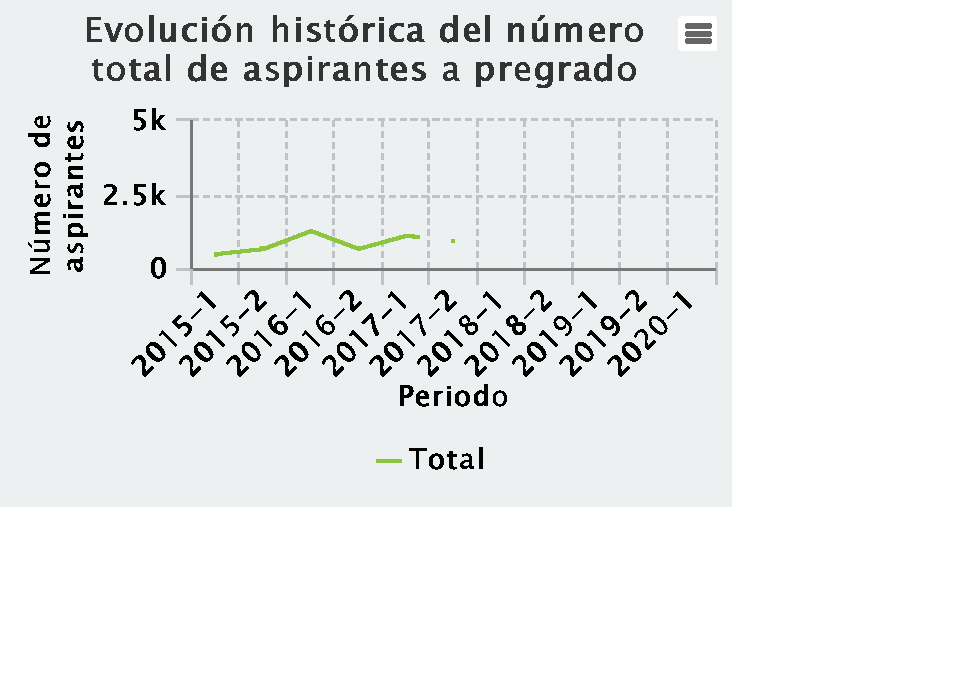
\includegraphics{BoletinTumaco_files/figure-latex/F1AspPre-1.pdf}

\hypertarget{informaciuxf3n-por-sexo}{%
\subsection{Información por sexo}\label{informaciuxf3n-por-sexo}}

A continuación, las figuras \ref{fig:F2AspPre} y \ref{fig:F3AspPre} presentan, respectivamente, la evolución histórica y el comportamiento actual del total de aspirantes a pregrado según el sexo biológico.

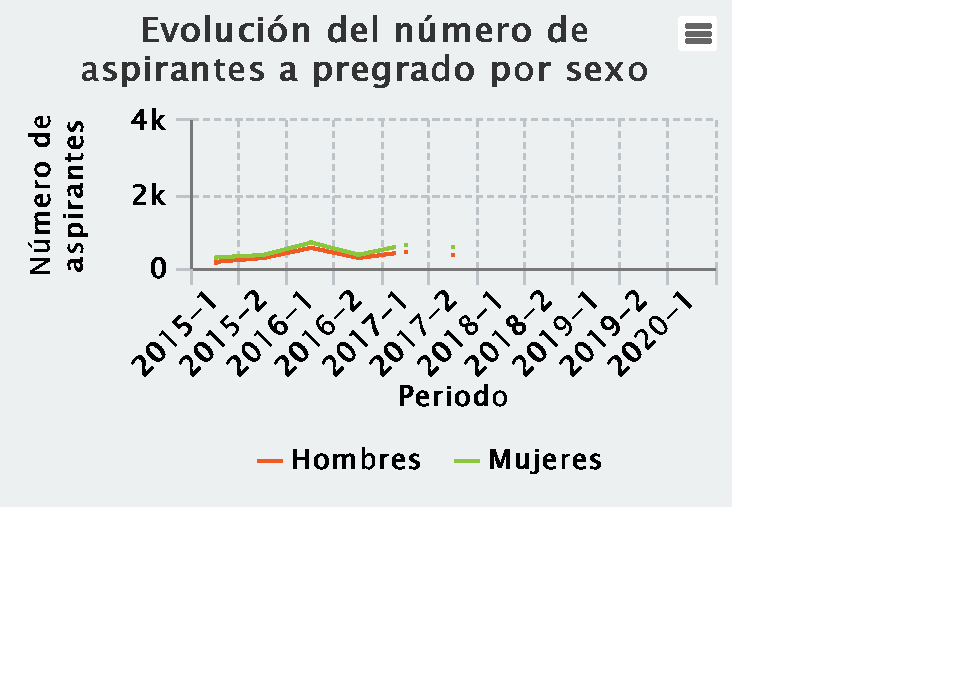
\includegraphics{BoletinTumaco_files/figure-latex/F2AspPre-1.pdf}
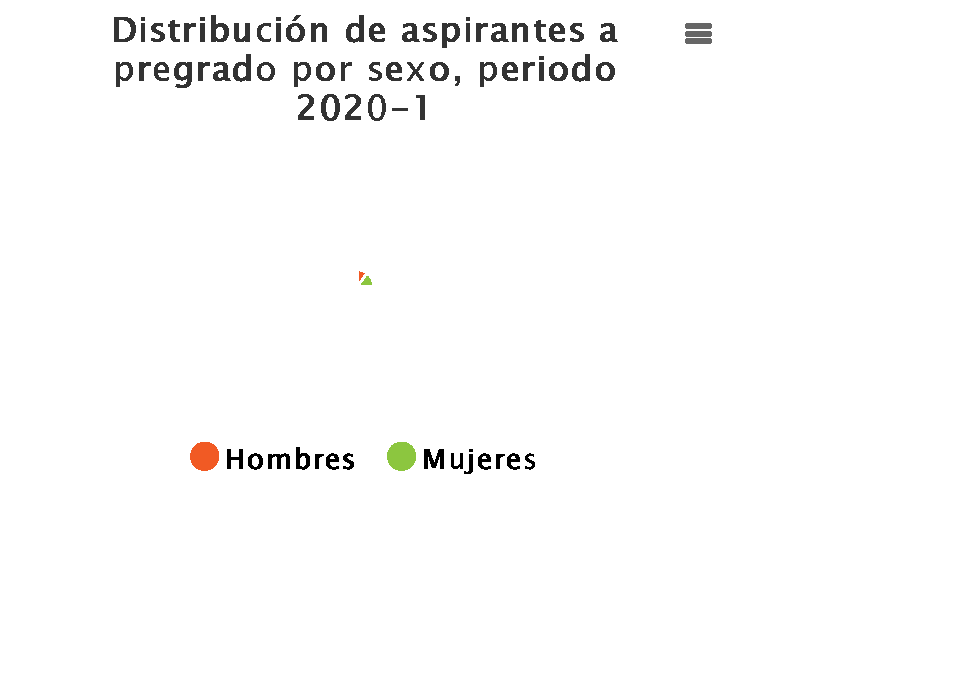
\includegraphics{BoletinTumaco_files/figure-latex/F3AspPre-1.pdf}

\hypertarget{informaciuxf3n-por-edad}{%
\subsection{Información por edad}\label{informaciuxf3n-por-edad}}

A continuación, las figuras \ref{fig:F4AspPre} y \ref{fig:F5AspPre} presentan, respectivamente, la evolución histórica y el comportamiento actual del total de aspirantes a pregrado por grupos de edad.

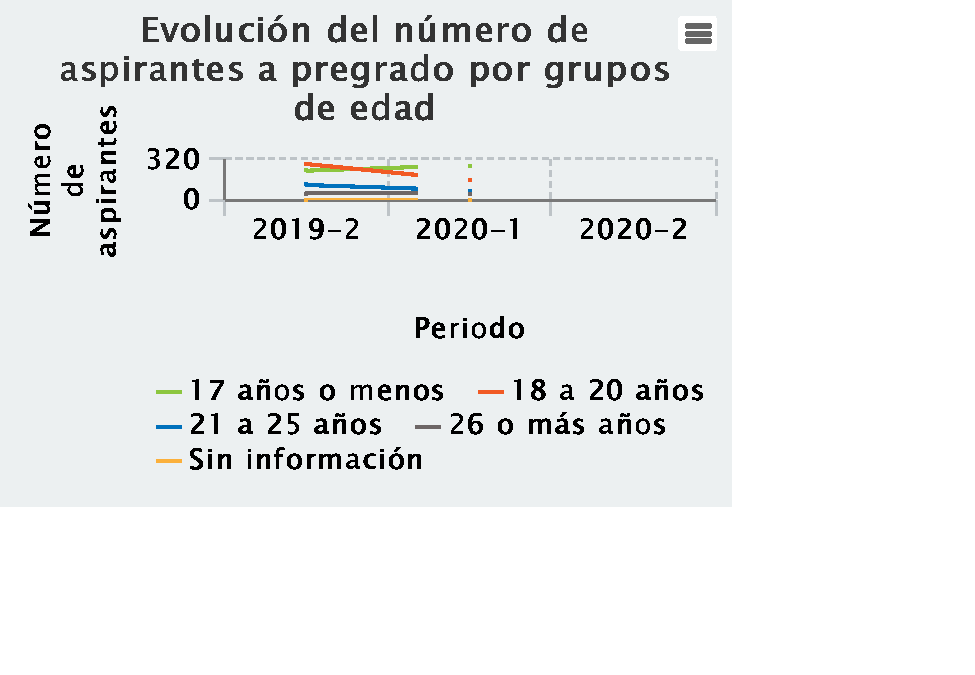
\includegraphics{BoletinTumaco_files/figure-latex/F4AspPre-1.pdf}
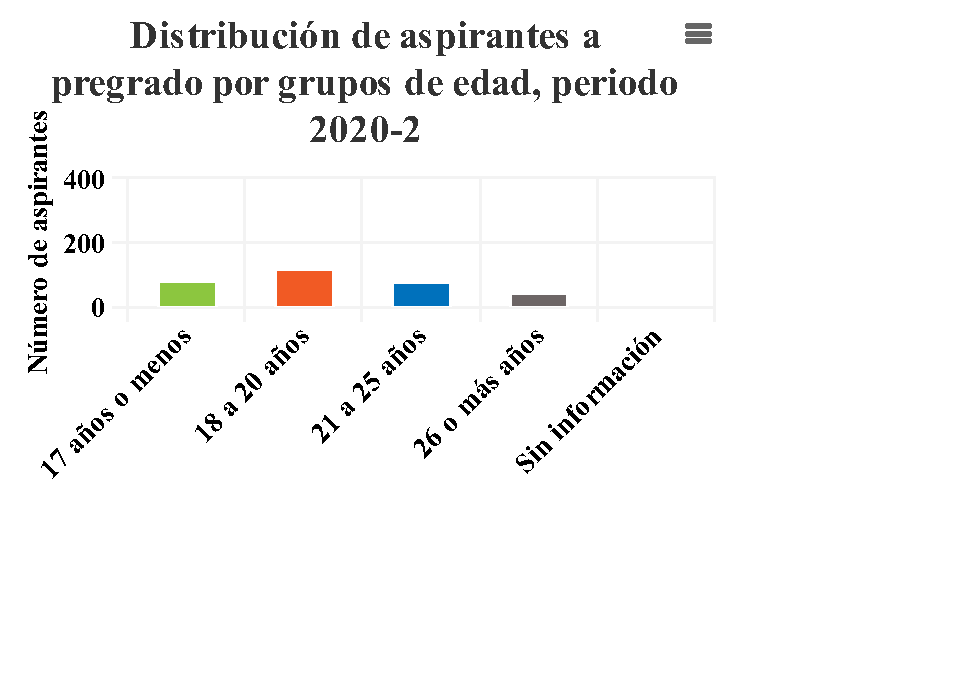
\includegraphics{BoletinTumaco_files/figure-latex/F5AspPre-1.pdf}

\hypertarget{informaciuxf3n-por-estrato-socioeconuxf3mico}{%
\subsection{Información por estrato socioeconómico}\label{informaciuxf3n-por-estrato-socioeconuxf3mico}}

A continuación, las figuras \ref{fig:F6AspPre} y \ref{fig:F7AspPre} presentan, respectivamente, la evolución histórica y el comportamiento actual del total de aspirantes a pregrado según el estrato socioeconómico de las viviendas en donde estos residen.

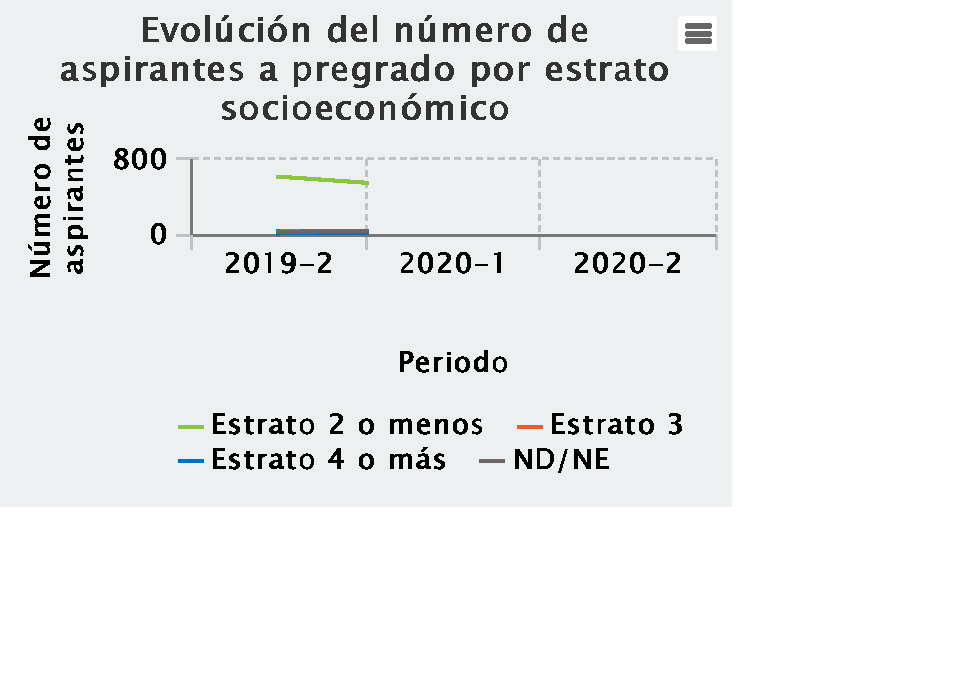
\includegraphics{BoletinTumaco_files/figure-latex/F6AspPre-1.pdf}
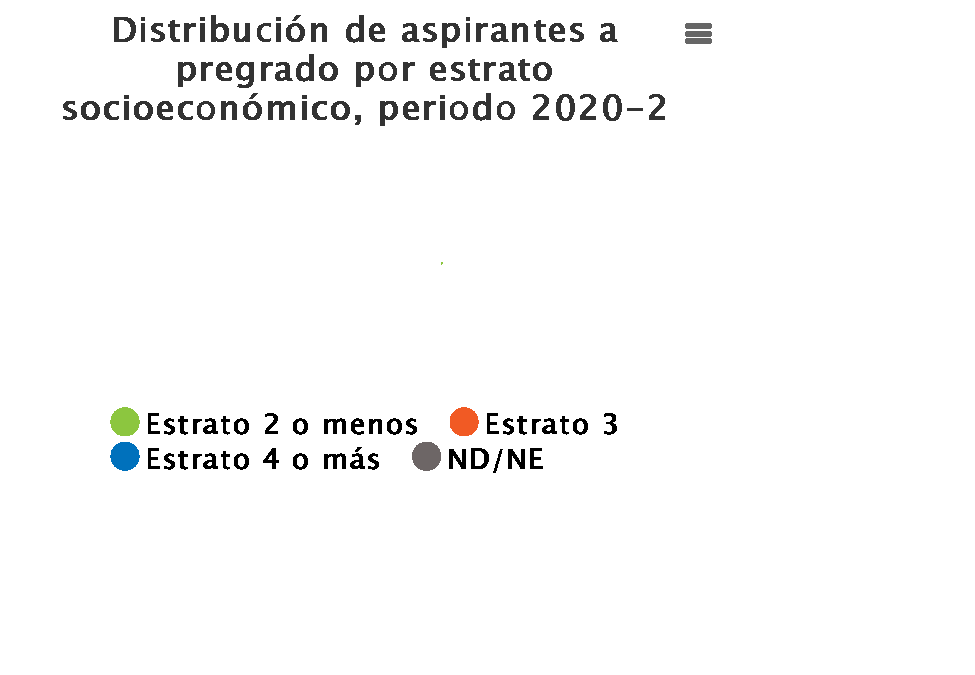
\includegraphics{BoletinTumaco_files/figure-latex/F7AspPre-1.pdf}

\hypertarget{tasa-de-absorciuxf3n}{%
\subsection{Tasa de absorción}\label{tasa-de-absorciuxf3n}}

A continuación, las figuras \ref{fig:F8AspPre} y \ref{fig:F9AspPre} presentan, respectivamente, la evolución histórica y el comportamiento actual del total de aspirantes admitidos a pregrado en la Sede Tumaco de la Universidad Nacional de Colombia.

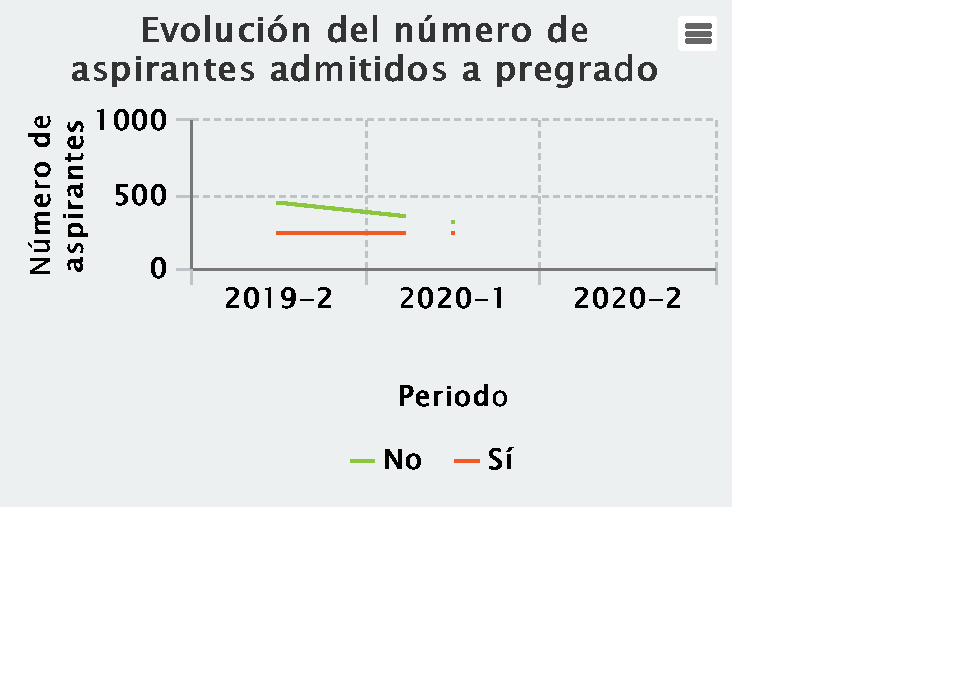
\includegraphics{BoletinTumaco_files/figure-latex/F8AspPre-1.pdf}
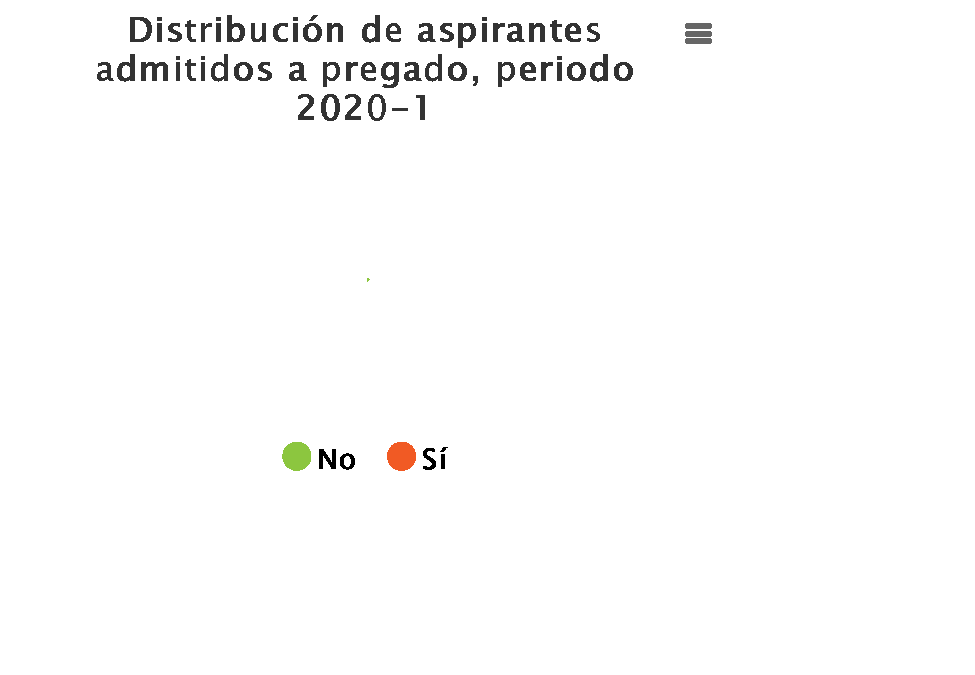
\includegraphics{BoletinTumaco_files/figure-latex/F9AspPre-1.pdf}

\hypertarget{tablas-cifras-agregadas}{%
\subsection{Tablas cifras agregadas}\label{tablas-cifras-agregadas}}

A continuación se presentan, a través de tablas, los agregados/consolidados históricos del total de aspirantes a pregrado de la Sede Tumaco por departamentos y municipios de procedencia.

Los interesados en \emph{imprimir}, \emph{copiar} o \emph{descargar} estas cifras, pueden hacerlo a través de las múltiples opciones que se ofrecen en la parte superior izquierda de cada una de las tablas que se presentan a continuación (Copiar, CSV, Excel, PDF e Imprimir). Así mismo estas tablas, dada su naturaleza web, permiten filtrar los resultados por aquellas variables de interés.

\hypertarget{departamentos-y-municipios-de-procedencia}{%
\subsubsection{Departamentos y municipios de procedencia}\label{departamentos-y-municipios-de-procedencia}}

A continuación, la tabla \ref{fig:F10AspPre} presenta el acumulado \textbf{histórico}, por \textbf{años y semestres}, de los aspirantes a pregrado por departamentos y municipios de procedencia en la Sede Tumaco.

\begin{figure}
\centering
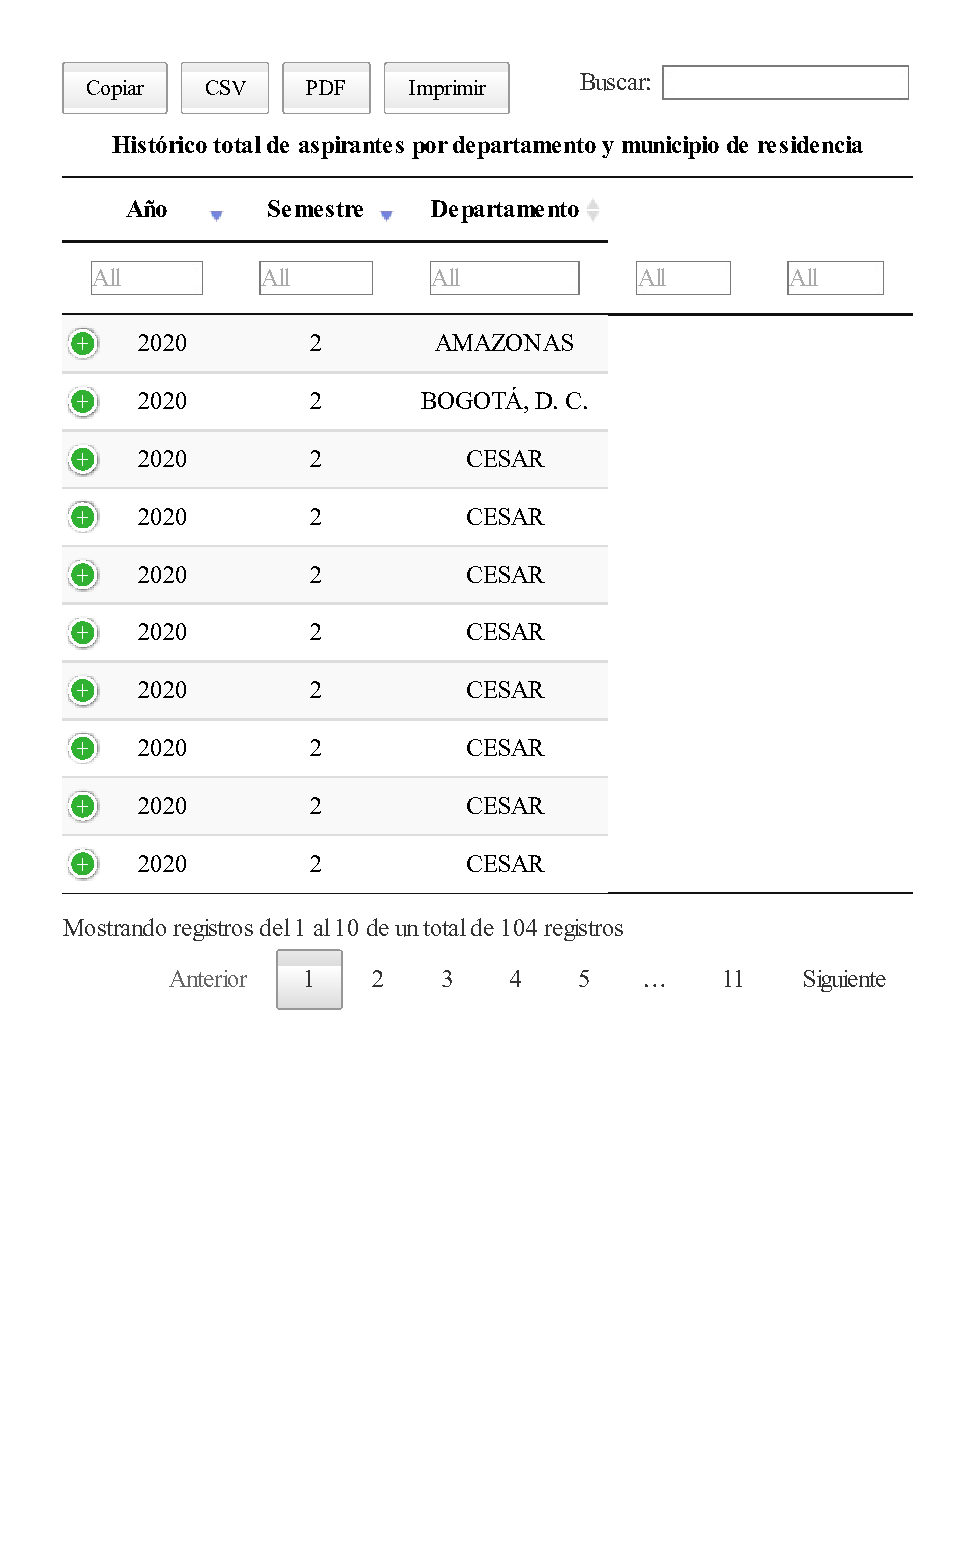
\includegraphics{BoletinTumaco_files/figure-latex/F10AspPre-1.pdf}
\caption{\label{fig:F10AspPre}Fuente: Dirección Nacional de Planeación y Estadística con base en información de la Dirección Nacional de Admisiones}
\end{figure}

\hypertarget{AdmPre}{%
\section{Admitidos a pregrado}\label{AdmPre}}

A continuación, se presentan las principales características asociadas a los admitidos a pregrado de la Sede Tumaco de la Universidad Nacional de Colombia. En específico, se presenta la evolución histórica de los admitidos a pregrado desde diferentes perspectivas: general, sexo, grupos de edad, estrato socioeconómico, departamentos y municipios de residencia así como los programas académicos, las facultades y las sedes andinas en las que estos se encuentran ubicados. Para cada una de las variables analizadas se presenta la evolución histórica (\emph{serie de tiempo}) así como el comportamiento actual (\emph{estado actual}) derivado de las últimas mediciones disponibles.

\hypertarget{evoluciuxf3n-histuxf3rica-1}{%
\subsection{Evolución Histórica}\label{evoluciuxf3n-histuxf3rica-1}}

A continuación, la Figura \ref{fig:F1AdmPre}, presenta la evolución histórica -\emph{desde el periodo 20151}-, del total de admitidos a pregrado en la sede.

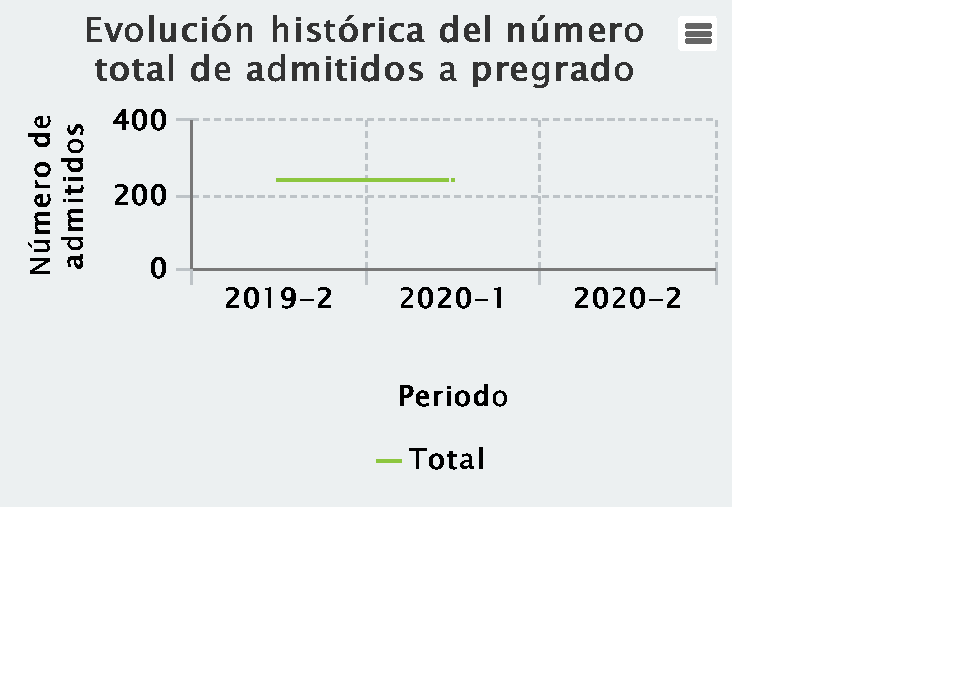
\includegraphics{BoletinTumaco_files/figure-latex/F1AdmPre-1.pdf}

\hypertarget{informaciuxf3n-por-sexo-1}{%
\subsection{Información por sexo}\label{informaciuxf3n-por-sexo-1}}

A continuación, las figuras \ref{fig:F2AdmPre} y \ref{fig:F3AdmPre} presentan, respectivamente, la evolución histórica y el comportamiento actual del total de admitidos a pregrado según el sexo biológico.

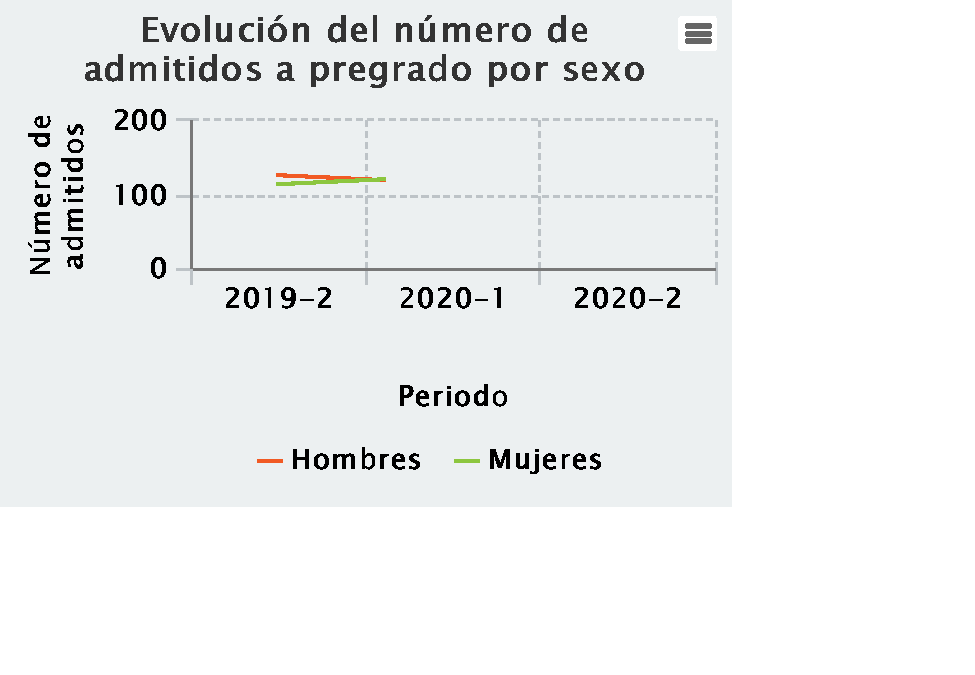
\includegraphics{BoletinTumaco_files/figure-latex/F2AdmPre-1.pdf}
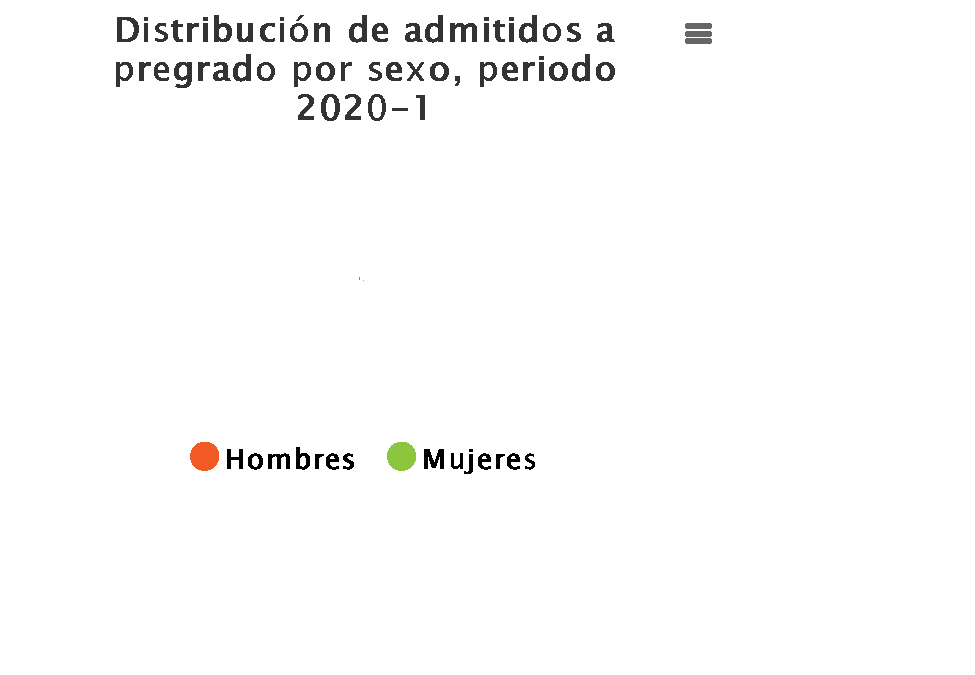
\includegraphics{BoletinTumaco_files/figure-latex/F3AdmPre-1.pdf}

\hypertarget{informaciuxf3n-por-edad-1}{%
\subsection{Información por edad}\label{informaciuxf3n-por-edad-1}}

A continuación, las figuras \ref{fig:F4AdmPre} y \ref{fig:F5AdmPre} presentan, respectivamente, la evolución histórica y el comportamiento actual del total de admitidos a pregrado por grupos de edad.

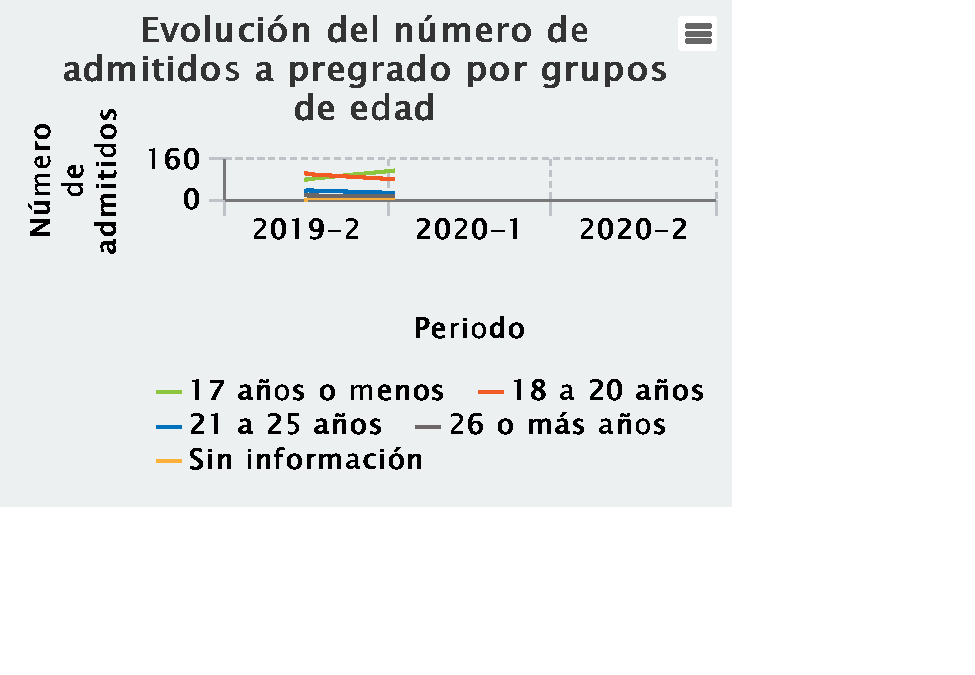
\includegraphics{BoletinTumaco_files/figure-latex/F4AdmPre-1.pdf}
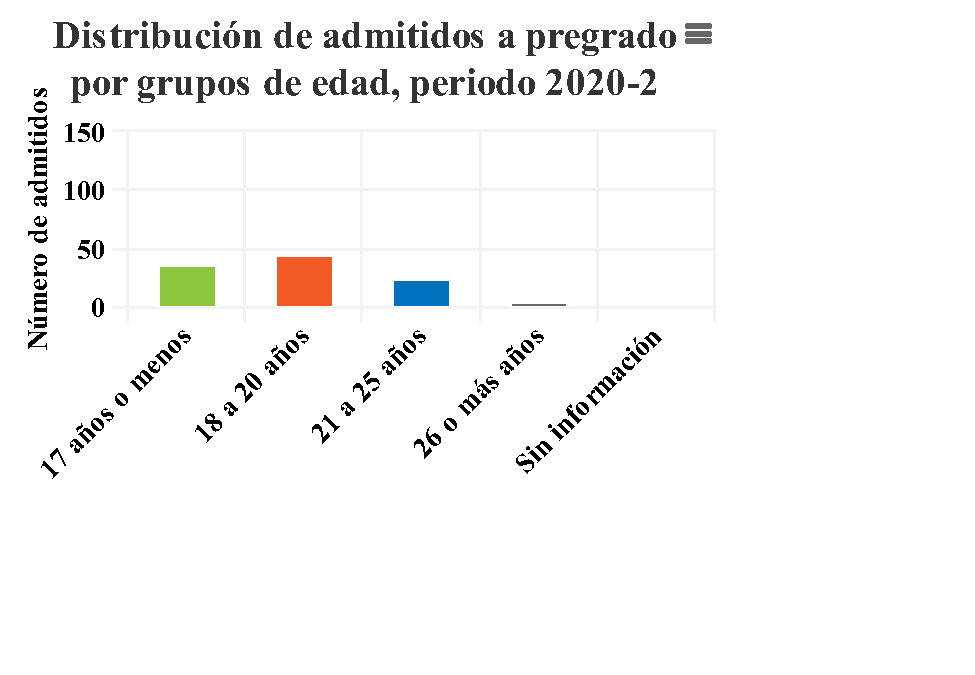
\includegraphics{BoletinTumaco_files/figure-latex/F5AdmPre-1.pdf}

\hypertarget{informaciuxf3n-por-estrato-socioeconuxf3mico-1}{%
\subsection{Información por estrato socioeconómico}\label{informaciuxf3n-por-estrato-socioeconuxf3mico-1}}

A continuación, las figuras \ref{fig:F6AdmPre} y \ref{fig:F7AdmPre} presentan, respectivamente, la evolución histórica y el comportamiento actual del total de admitidos a pregrado según el estrato socioeconómico de las viviendas en donde estos residen.

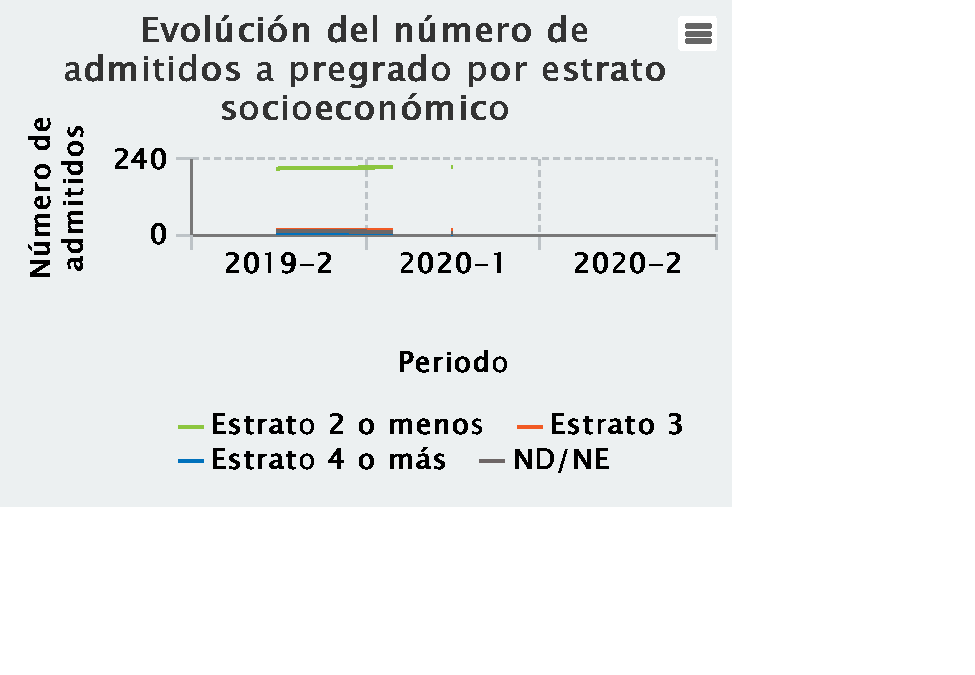
\includegraphics{BoletinTumaco_files/figure-latex/F6AdmPre-1.pdf}
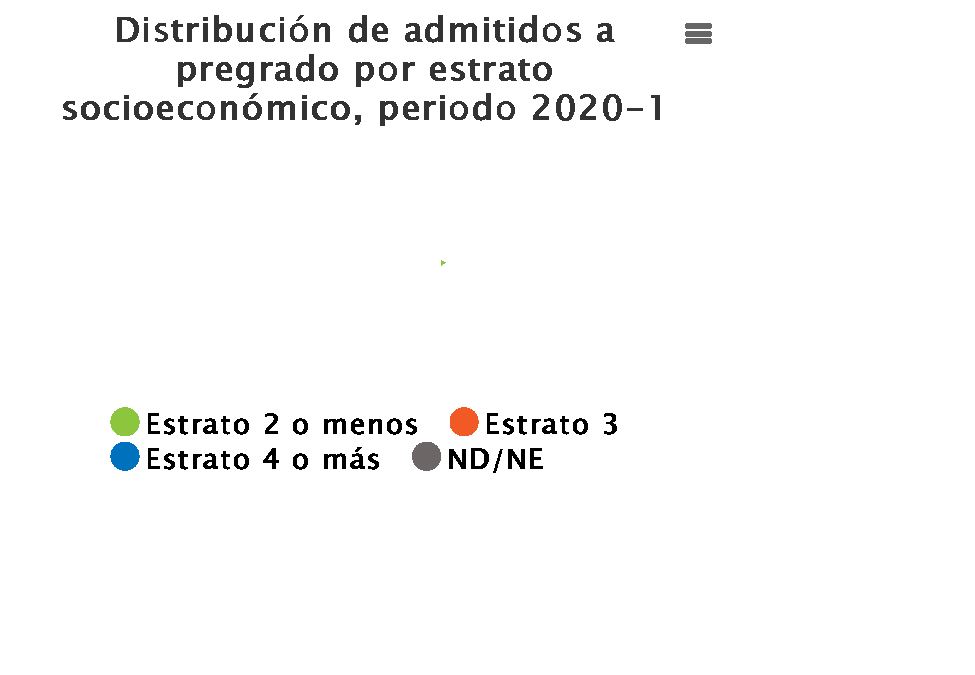
\includegraphics{BoletinTumaco_files/figure-latex/F7AdmPre-1.pdf}

\hypertarget{tablas-cifras-agregadas-1}{%
\subsection{Tablas cifras agregadas}\label{tablas-cifras-agregadas-1}}

A continuación se presentan, a través de tablas, los agregados/consolidados históricos del total de admitidos a pregrado de la Sede Tumaco por departamentos y municipios de procedencia, así como los programas académicos y las sedes andinas a las que estos pertecenecen.

Los interesados en \emph{imprimir}, \emph{copiar} o \emph{descargar} estas cifras, pueden hacerlo a través de las múltiples opciones que se ofrecen en la parte superior izquierda de cada una de las tablas que se presentan a continuación (Copiar, CSV, Excel, PDF e Imprimir). Así mismo estas tablas, dada su naturaleza web, permiten filtrar los resultados por aquellas variables de interés.

\hypertarget{departamentos-y-municipios-de-procedencia.}{%
\subsubsection{Departamentos y municipios de procedencia.}\label{departamentos-y-municipios-de-procedencia.}}

A continuación, la tabla \ref{fig:F8AdmPre} presenta el acumulado \textbf{histórico}, por \textbf{años y semestres}, en la Sede Tumaco de los admitidos a pregrado por departamentos y municipios de procedencia.

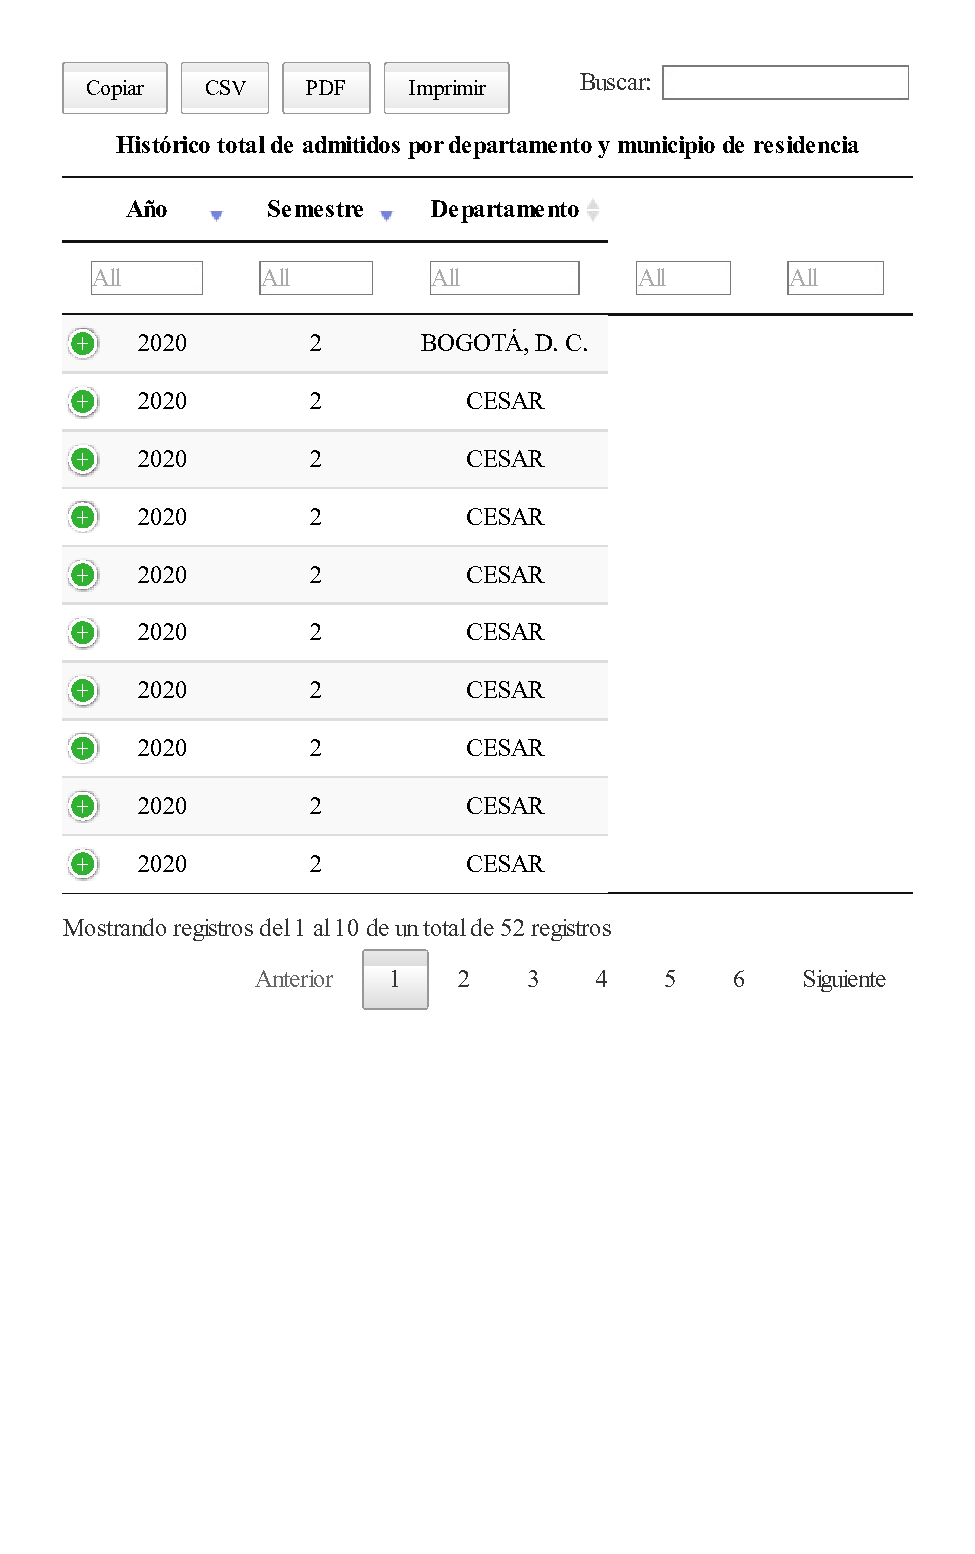
\includegraphics{BoletinTumaco_files/figure-latex/F8AdmPre-1.pdf}

\hypertarget{programas-acaduxe9micos-de-pregrado}{%
\subsubsection{Programas académicos de pregrado}\label{programas-acaduxe9micos-de-pregrado}}

A continuación, la tabla \ref{fig:F9AdmPre} presenta el acumulado \textbf{histórico}, por \textbf{años y semestres}, en la Sede Tumaco de los admitidos a pregrado por programas académicos y sedes andinas en las que estos se encuentran adscritos.

\begin{figure}
\centering
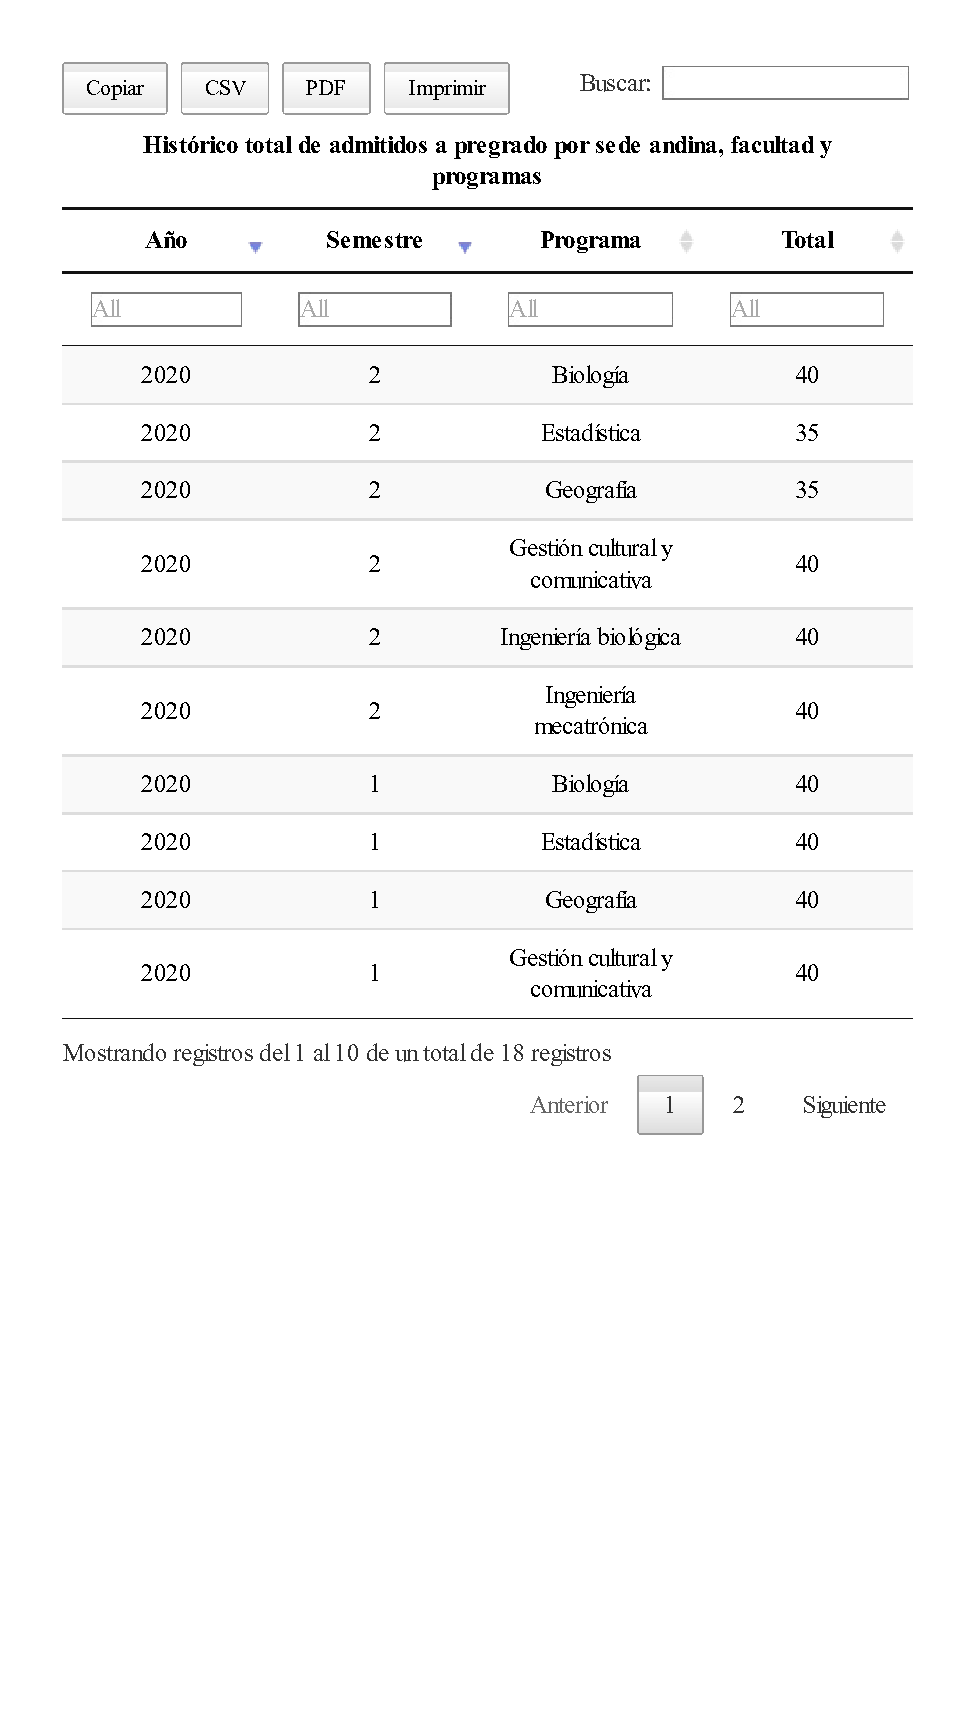
\includegraphics{BoletinTumaco_files/figure-latex/F9AdmPre-1.pdf}
\caption{\label{fig:F9AdmPre}Fuente: Dirección Nacional de Planeación y Estadística con base en información de la Dirección Nacional de Admisiones}
\end{figure}

\hypertarget{Estudiantes}{%
\chapter{Estudiantes}\label{Estudiantes}}

Este capítulo presenta el consolidado de las principales características asociadas a la información estadística oficial de los estudiantes matriculados en pregrado en la sede Tumaco de la Universidad Nacional de Colombia. A continuación, se presenta una breve descripción de las secciones que hacen parte de este capítulo así como la ubicación del sitio web en donde se presentan las definiciones, los estándares y las codificaciones/clasificaciones que hacen parte de la información acá contenida (\emph{metadatos}) y cuya exploración y lectura, sin duda, facilitará el entendimiento de las cifras asociadas a las poblaciones de estudiantes matriculados.

La Sede Tumaco en la actualidad no cuenta con programas de postgrado. Por lo anterior, en este capítulo no se dispone información estadística para este nivel de formación.

\textbf{Secciones}

El proceso de formación en pregrado en la Sede Tumaco se da a la luz de los lineamientos definidos en el Programa Especial de Admisión y Movilidad Académica el cual, como se presenta en la sección \protect\hyperlink{peama}{PEAMA} del presente boletín, consta de tres etapas: \emph{etapa inicial}, \emph{etapa de movilidad} y \emph{etapa final}. Teniendo en cuenta lo anterior, en este capítulo se presentan las estadísticas oficiales asociadas a tres poblaciones de estudiantes matriculados en pregrado en la Sede Tumaco de la Universidad Nacional de Colombia.

\begin{itemize}
\item
  \protect\hyperlink{MatPre}{Matriculados en pregrado}: contiene la información oficial del total de estudiantes matricualdos en pregrado en la Universidad y que han sido admitidos a través de la Sede Tumaco. Incluye los estudiantes de pregrado que se encuentran en las tres etapas de formación: \emph{inicial}, \emph{movilidad} y \emph{final}.
\item
  \protect\hyperlink{MatPreIni}{Matriculados en pregrado etapa inicial}: contiene la información oficial del total de estudiantes matriculados en pregrado en la Universidad, que han sido admitidos a través de la Sede Tumaco y que encuentran en la etapa inicial de su proceso de formación académica. Es decir, hace referencia a los estudiantes de pregrado que se encuentran ubicados de manera fisíca en el campus de la Sede Tumaco.
\item
  \protect\hyperlink{MatPreMov}{Matriculados en pregrado etapa movilidad}: contiene la información oficial del total de estudiantes matriculados en pregrado en la Universidad, que han sido admitidos a través de la Sede Tumaco y que encuentran en la etapa de movilidad en su proceso de formación académica. Es decir, hace referencia a los estudiantes de pregrado, admitidos a través de la Sede Tumaco y que se encuentran cursando sus estudios en los campus de las sedes Bogotá, Medellín, Manizales o Palmira.
\end{itemize}

\textbf{Metadatos}

La construcción de las cifras oficiales de estudiantes matriculados en pregrado de la Sede Tumaco, las definiciones que hacen parte de estas así como las codificaciones y clasificaciones aquí empleadas se encuentran contenidas en la sección \textbf{Matriculados} del capítulo de \emph{Metadatos} de las cifras oficiales generales que hacen parte de la página de \href{http://estadisticas.unal.edu.co/home/}{estadísticas} de la Universidad Nacional de Colombia. Invitamos a los lectores a explorar y conocer estos metadatos los cuales, además de orientar y facilitar el entendimiento de la información acá expuesta, se encuentran disponibles en el siguiente enlace.

\begin{itemize}
\tightlist
\item
  \href{http://estadisticas.unal.edu.co/menu-principal/cifras-generales/metadatos/cifras-generales/}{Metadatos Cifras Oficiales Universidad Nacional de Colombia}
\end{itemize}

\hypertarget{MatPre}{%
\section{Matriculados en pregrado}\label{MatPre}}

A continuación, se presenta la información oficial del total de estudiantes matricualdos en pregrado en la Universidad y que han sido admitidos a través de la \textbf{Sede Tumaco}. Incluye los estudiantes de pregrado que se encuentran en las tres etapas de formación: \emph{inicial}, \emph{movilidad} y \emph{final}. En específico, se presenta la evolución histórica de los matriculados en pregrado desde diferentes perspectivas: general, etapa de formación, sedes andinas, sexo, grupos de edad, estrato socioeconómico, departamentos y municipios de residencia y programas académicos en los que estos se encuentran matriculados. Para cada una de las variables analizadas se presenta la evolución histórica (\emph{serie de tiempo}) así como el comportamiento actual (\emph{estado actual}) derivado de las últimas mediciones disponibles.

\hypertarget{evoluciuxf3n-histuxf3rica-2}{%
\subsection{Evolución histórica}\label{evoluciuxf3n-histuxf3rica-2}}

A continuación, la Figura \ref{fig:F1MatPre}, presenta la evolución histórica -\emph{desde el periodo 20151}-, del total de matriculados en pregrado en la \textbf{Sede Tumaco}.

\begin{figure}
\centering
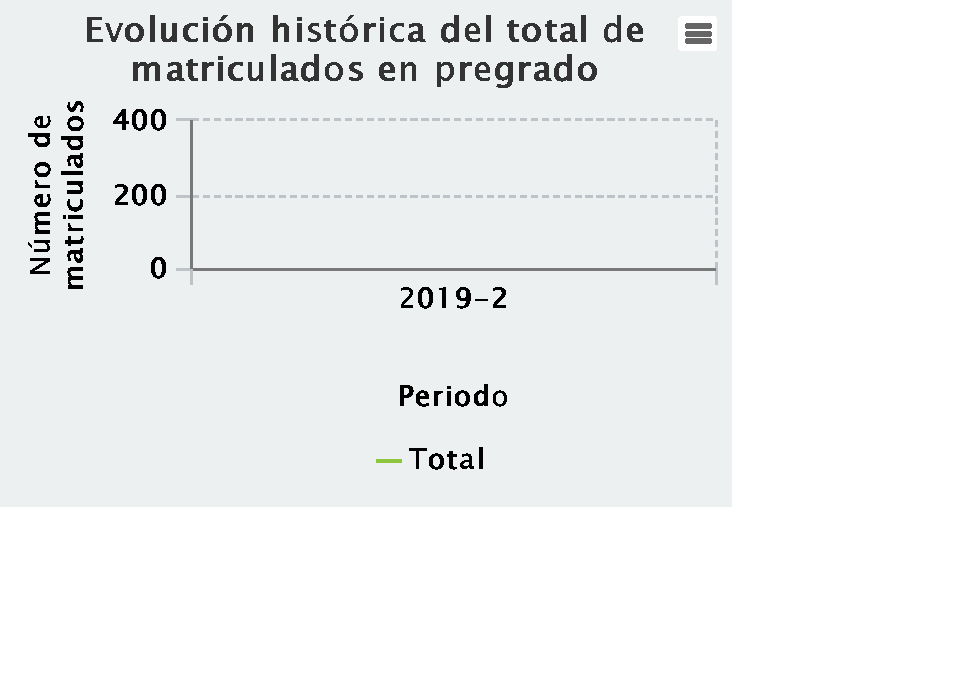
\includegraphics{BoletinTumaco_files/figure-latex/F1MatPre-1.pdf}
\caption{\label{fig:F1MatPre}Fuente: Dirección Nacional de Planeación y Estadística con base en información de la Dirección Nacional Información Académica}
\end{figure}

\hypertarget{informaciuxf3n-por-etapa-de-formaciuxf3n}{%
\subsection{Información por etapa de formación}\label{informaciuxf3n-por-etapa-de-formaciuxf3n}}

A continuación, las figuras \ref{fig:F2MatPre} y \ref{fig:F3MatPre} presentan, respectivamente, la evolución histórica y el comportamiento actual del total de matriculados en pregrado en la \textbf{Sede Tumaco} según la etapa de formación en la que estos se encuentran.

\begin{itemize}
\item
  \emph{Etapa Inicial}: Estudiantes matriculados en pregrado ubicados físicamente en la \emph{Sede Tumaco}
\item
  \emph{Etapa de movilidad}: Estudiantes matriculados en pregrado ubicados físicamente en las sedes andinas (\emph{Bogotá}, \emph{Medellín}, \emph{Manizales} o \emph{Palmira}).
\end{itemize}

\begin{figure}
\centering
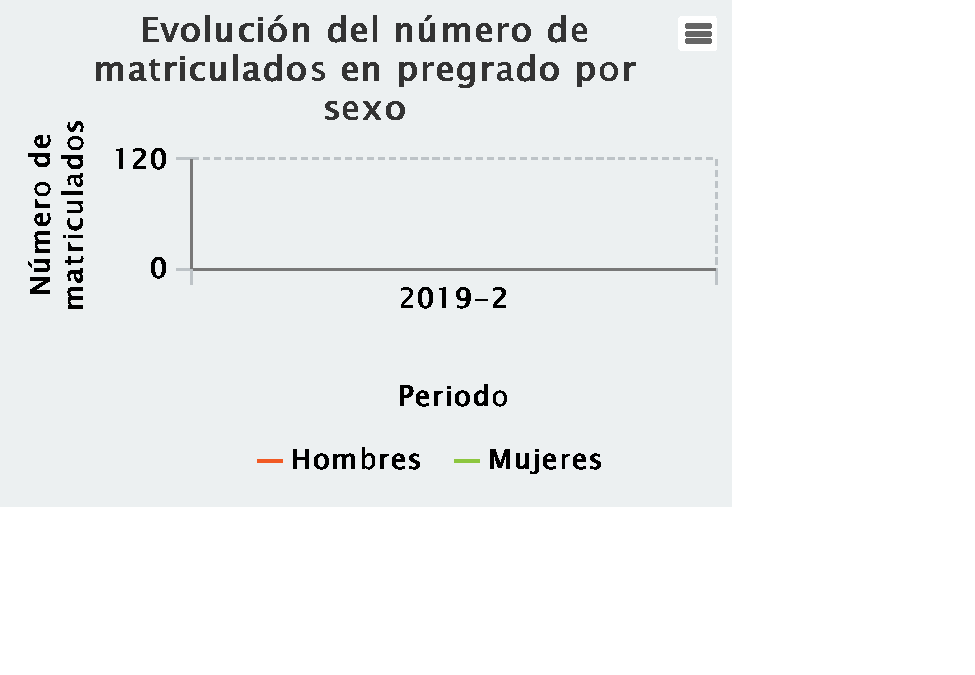
\includegraphics{BoletinTumaco_files/figure-latex/F2MatPre-1.pdf}
\caption{\label{fig:F2MatPre}Fuente: Dirección Nacional de Planeación y Estadística con base en información de la Dirección Nacional Información Académica}
\end{figure}

\begin{figure}
\centering
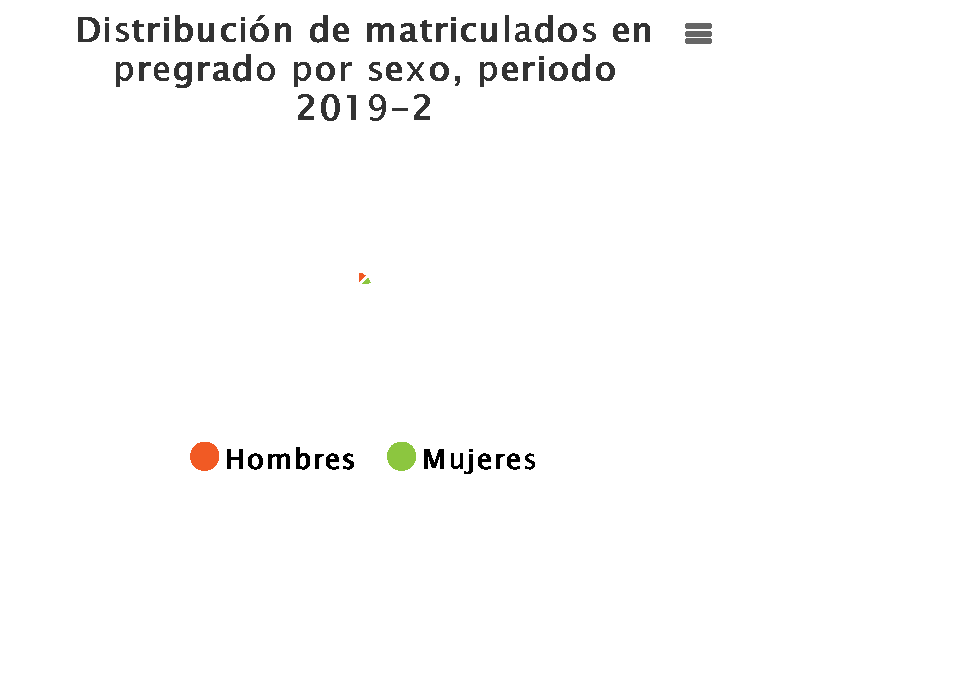
\includegraphics{BoletinTumaco_files/figure-latex/F3MatPre-1.pdf}
\caption{\label{fig:F3MatPre}Fuente: Dirección Nacional de Planeación y Estadística con base en información de la Dirección Nacional Información Académica}
\end{figure}

\hypertarget{informaciuxf3n-por-sede-andina}{%
\subsection{Información por sede andina}\label{informaciuxf3n-por-sede-andina}}

A continuación, las figuras \ref{fig:F4MatPre} y \ref{fig:F5MatPre} presentan, respectivamente, la evolución histórica y el comportamiento actual del total de estudiantes matriculados de pregrado en la \textbf{Sede Tumaco} según la sede andina en la que estos cursarán (etapa inicial) o se encuentran cursando sus estudios (etapa de movilidad).

\begin{figure}
\centering
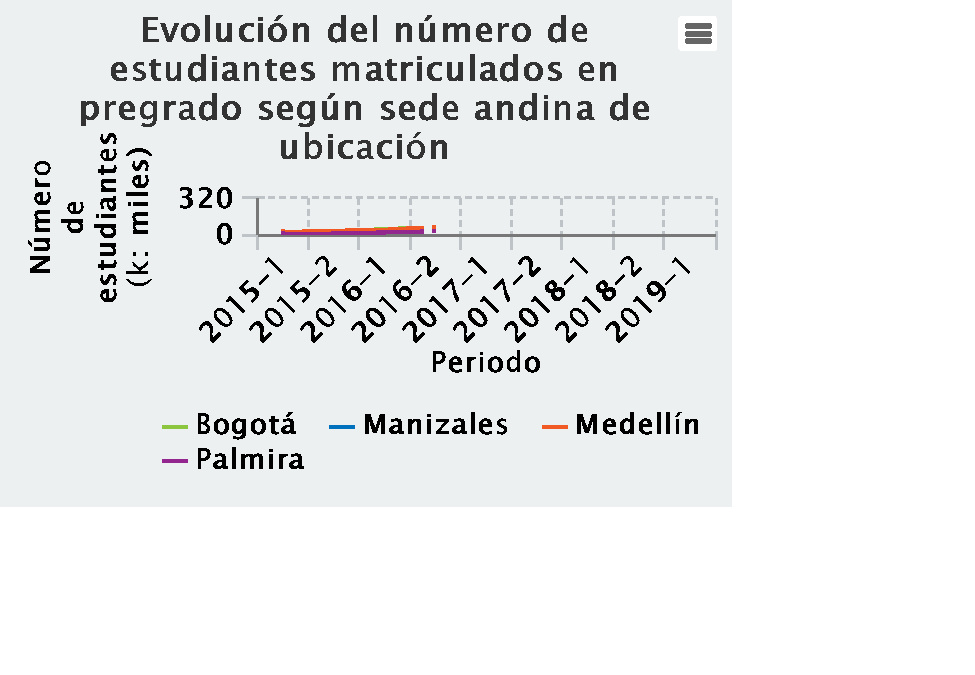
\includegraphics{BoletinTumaco_files/figure-latex/F4MatPre-1.pdf}
\caption{\label{fig:F4MatPre}Fuente: Dirección Nacional de Planeación y Estadística con base en información de la Dirección Nacional Información Académica}
\end{figure}

\begin{figure}
\centering
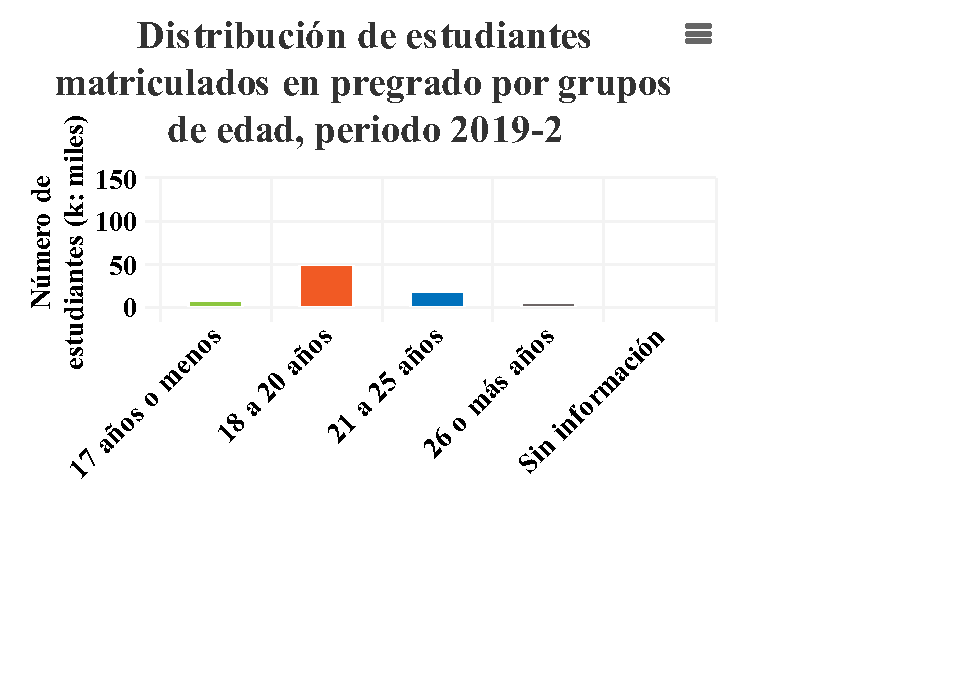
\includegraphics{BoletinTumaco_files/figure-latex/F5MatPre-1.pdf}
\caption{\label{fig:F5MatPre}Fuente: Dirección Nacional de Planeación y Estadística con base en información de la Dirección Nacional Información Académica}
\end{figure}

\hypertarget{informaciuxf3n-por-sexo-2}{%
\subsection{Información por sexo}\label{informaciuxf3n-por-sexo-2}}

A continuación, las figuras \ref{fig:F6MatPre} y \ref{fig:F7MatPre} presentan, respectivamente, la evolución histórica y el comportamiento actual del total de matriculados en pregrado en la \textbf{Sede Tumaco} según el sexo biológico.

\begin{figure}
\centering
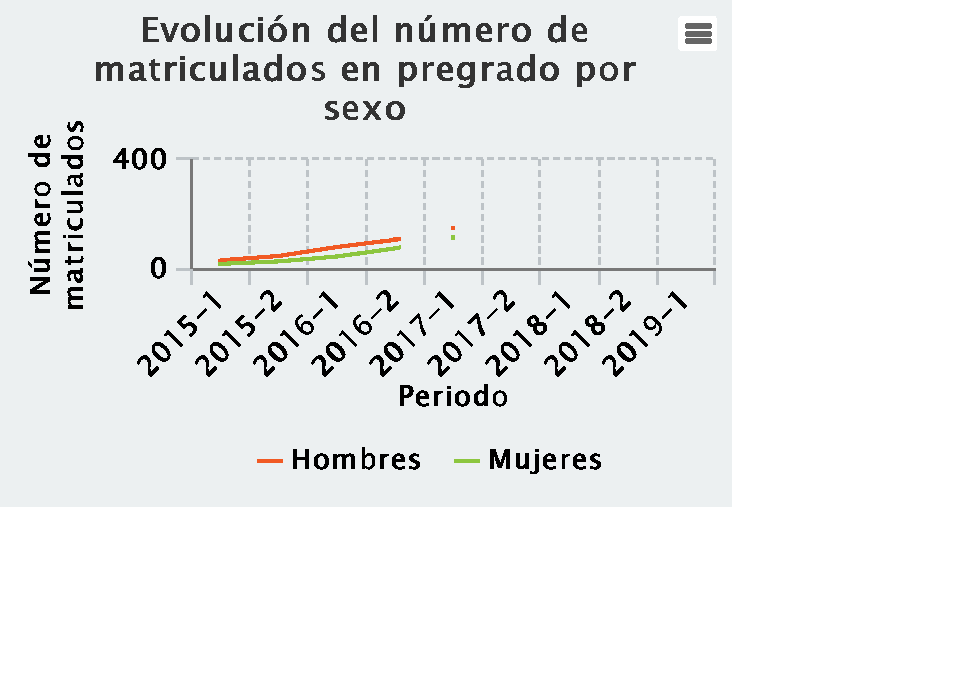
\includegraphics{BoletinTumaco_files/figure-latex/F6MatPre-1.pdf}
\caption{\label{fig:F6MatPre}Fuente: Dirección Nacional de Planeación y Estadística con base en información de la Dirección Nacional Información Académica}
\end{figure}

\begin{figure}
\centering
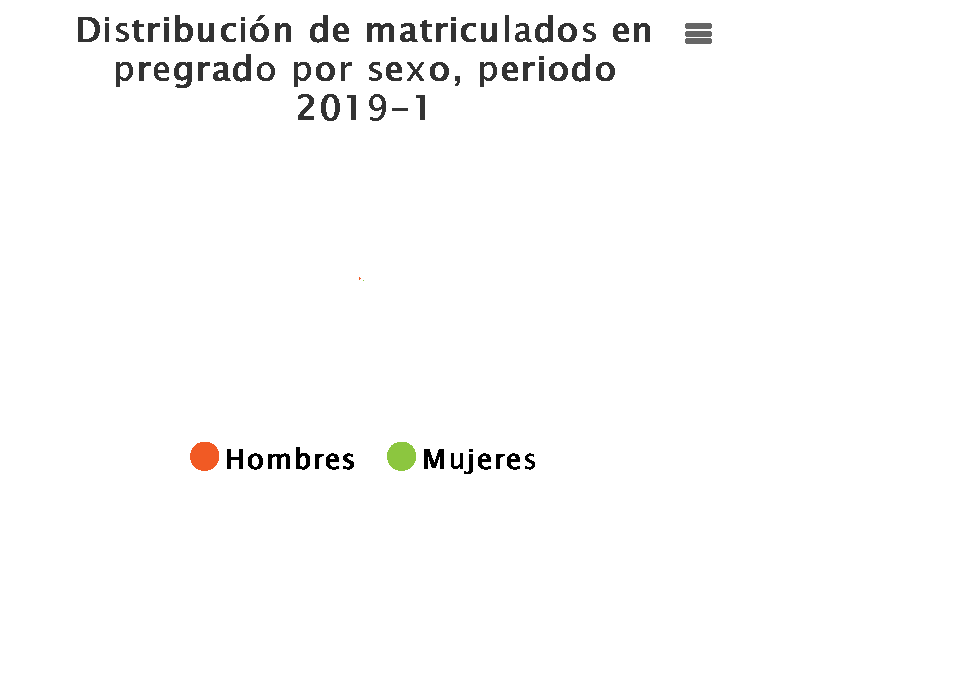
\includegraphics{BoletinTumaco_files/figure-latex/F7MatPre-1.pdf}
\caption{\label{fig:F7MatPre}Fuente: Dirección Nacional de Planeación y Estadística con base en información de la Dirección Nacional Información Académica}
\end{figure}

\hypertarget{informaciuxf3n-por-edad-2}{%
\subsection{Información por edad}\label{informaciuxf3n-por-edad-2}}

A continuación, las figuras \ref{fig:F8MatPre} y \ref{fig:F9MatPre} presentan, respectivamente, la evolución histórica y el comportamiento actual del total de estudiantes matriculados en pregrado de la \textbf{Sede Tumaco} según grupos de edad.

\begin{figure}
\centering
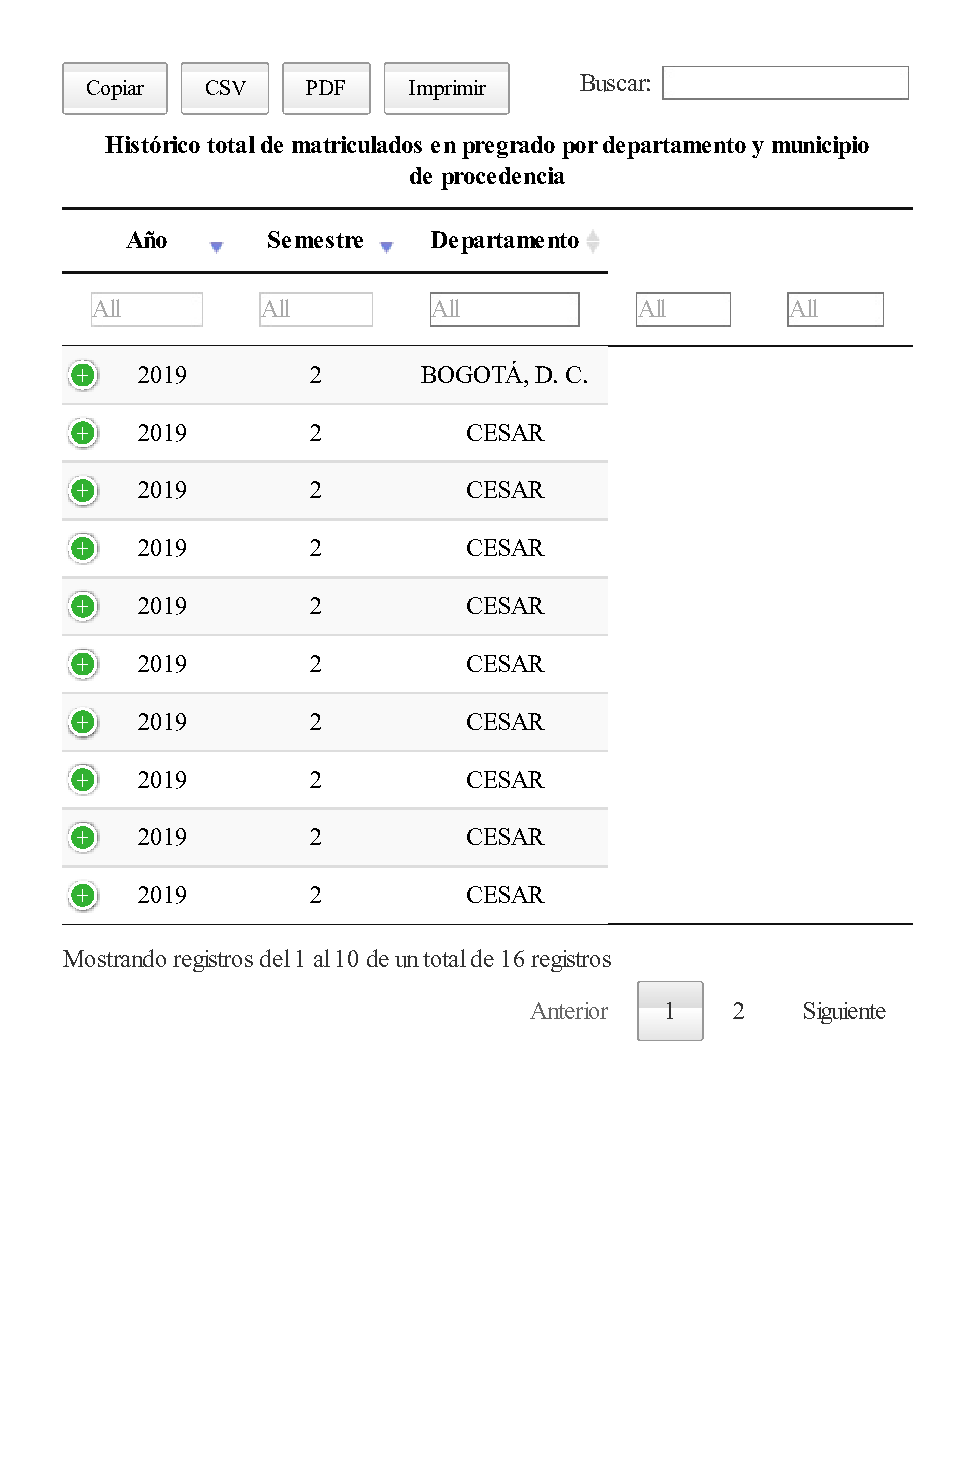
\includegraphics{BoletinTumaco_files/figure-latex/F8MatPre-1.pdf}
\caption{\label{fig:F8MatPre}Fuente: Dirección Nacional de Planeación y Estadística con base en información de la Dirección Nacional Información Académica}
\end{figure}

\begin{figure}
\centering
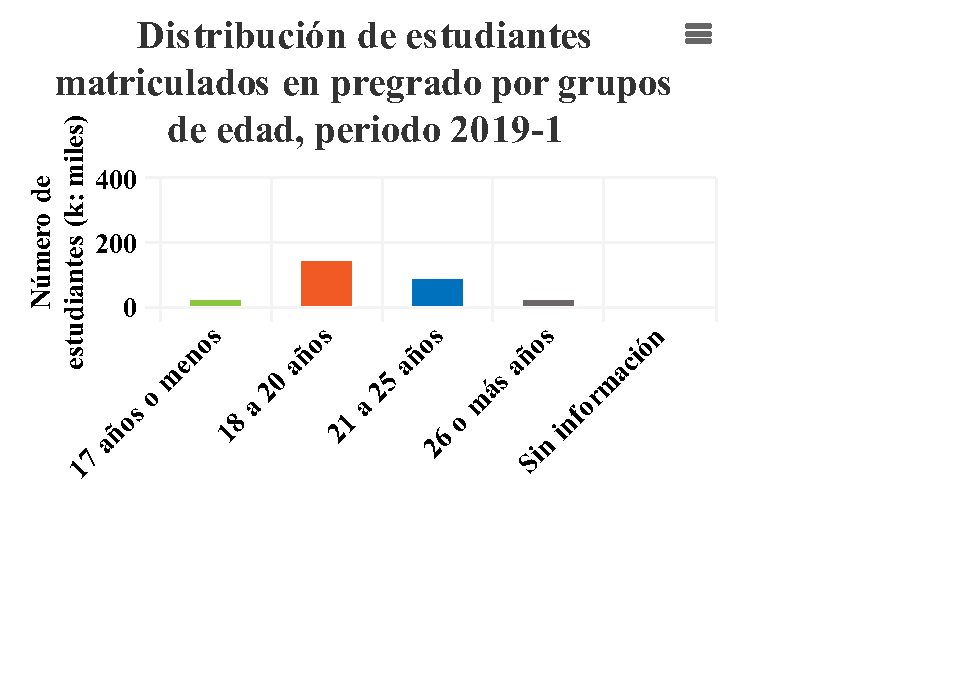
\includegraphics{BoletinTumaco_files/figure-latex/F9MatPre-1.pdf}
\caption{\label{fig:F9MatPre}Fuente: Dirección Nacional de Planeación y Estadística con base en información de la Dirección Nacional Información Académica}
\end{figure}

\hypertarget{informaciuxf3n-por-estrato}{%
\subsection{Información por estrato}\label{informaciuxf3n-por-estrato}}

A continuación, las figuras \ref{fig:F10MatPre} y \ref{fig:F11MatPre} presentan, respectivamente, la evolución histórica y el comportamiento actual del total de estudiantes matriculados en pregrado en la \textbf{Sede Tumaco} según el estrato socioeconómico.

\begin{figure}
\centering
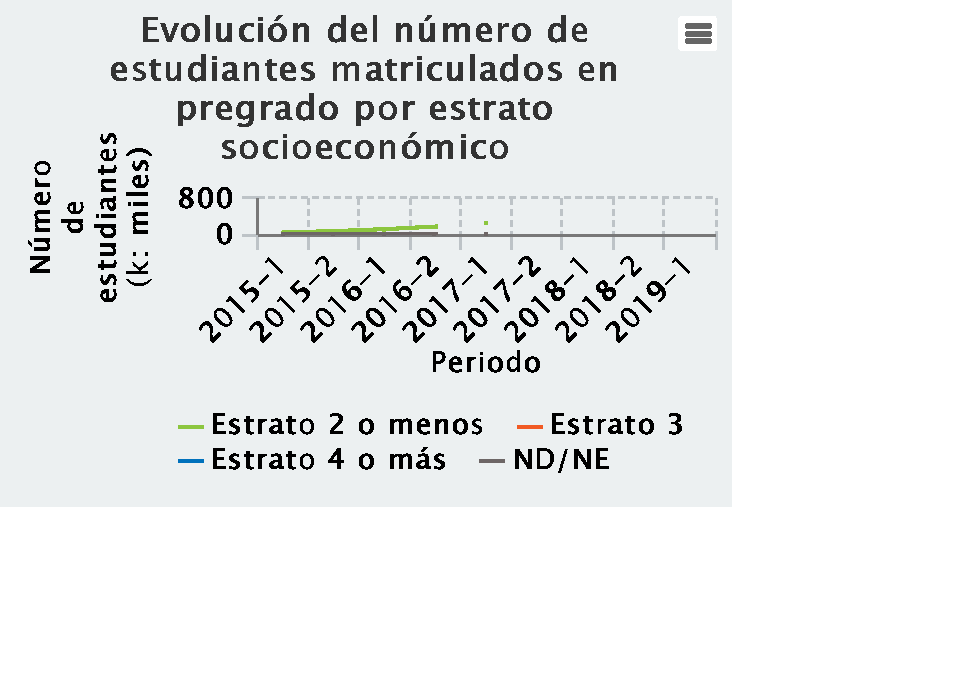
\includegraphics{BoletinTumaco_files/figure-latex/F10MatPre-1.pdf}
\caption{\label{fig:F10MatPre}Fuente: Dirección Nacional de Planeación y Estadística con base en información de la Dirección Nacional Información Académica}
\end{figure}

\begin{figure}
\centering
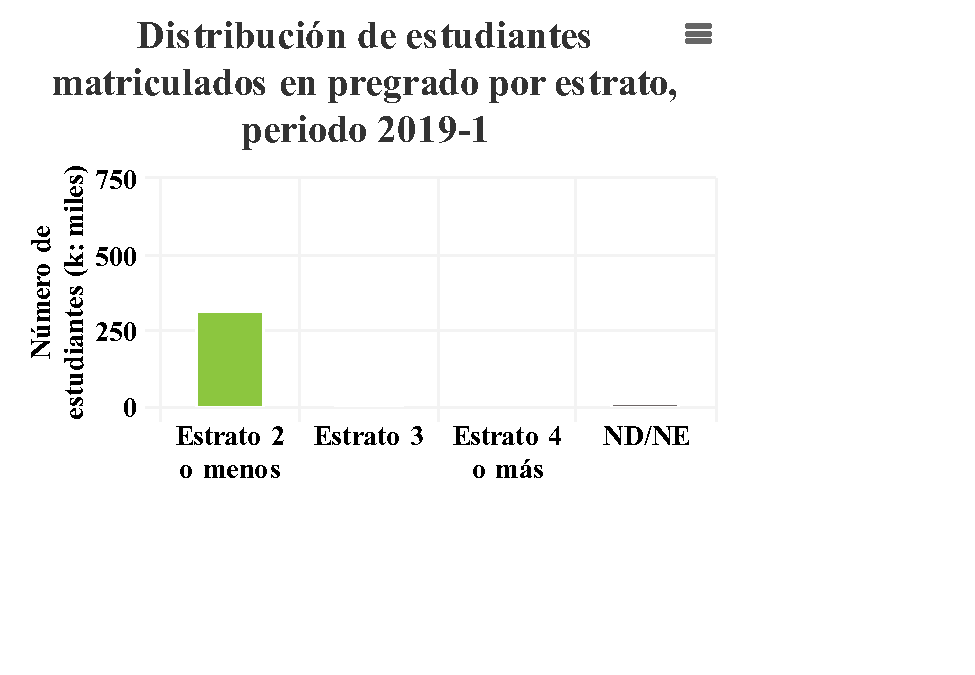
\includegraphics{BoletinTumaco_files/figure-latex/F11MatPre-1.pdf}
\caption{\label{fig:F11MatPre}Fuente: Dirección Nacional de Planeación y Estadística con base en información de la Dirección Nacional Información Académica}
\end{figure}

\hypertarget{tablas-cifras-agregadas-2}{%
\subsection{Tablas cifras agregadas}\label{tablas-cifras-agregadas-2}}

A continuación se presentan, a través de tablas, los agregados/consolidados históricos del total de matriculados en pregrado de la \textbf{Sede Tumaco} por departamentos y municipios de procedencia así como los programas académicos de pregrado que estos cursan en las sedes andinas de la Universidad (Bogotá, Medellín, Manizales y Palmira).

Los interesados en \emph{imprimir}, \emph{copiar} o \emph{descargar} estas cifras, pueden hacerlo a través de las múltiples opciones que se ofrecen en la parte superior izquierda de cada una de las tablas (Copiar, CSV, Excel, PDF e Imprimir). Así mismo, estas tablas permiten filtrar los resultados por aquellas variables de interés.

\hypertarget{departamentos-y-municipios-de-procedencia-1}{%
\subsubsection{Departamentos y municipios de procedencia}\label{departamentos-y-municipios-de-procedencia-1}}

A continuación, la Tabla \ref{fig:F12MatPre} presenta los acumulados \textbf{históricos}, por \textbf{años y semestres}, en la \textbf{Sede Tumaco}, de los matriculados en pregrado por departamentos y municipios de procedencia.

\begin{figure}
\centering
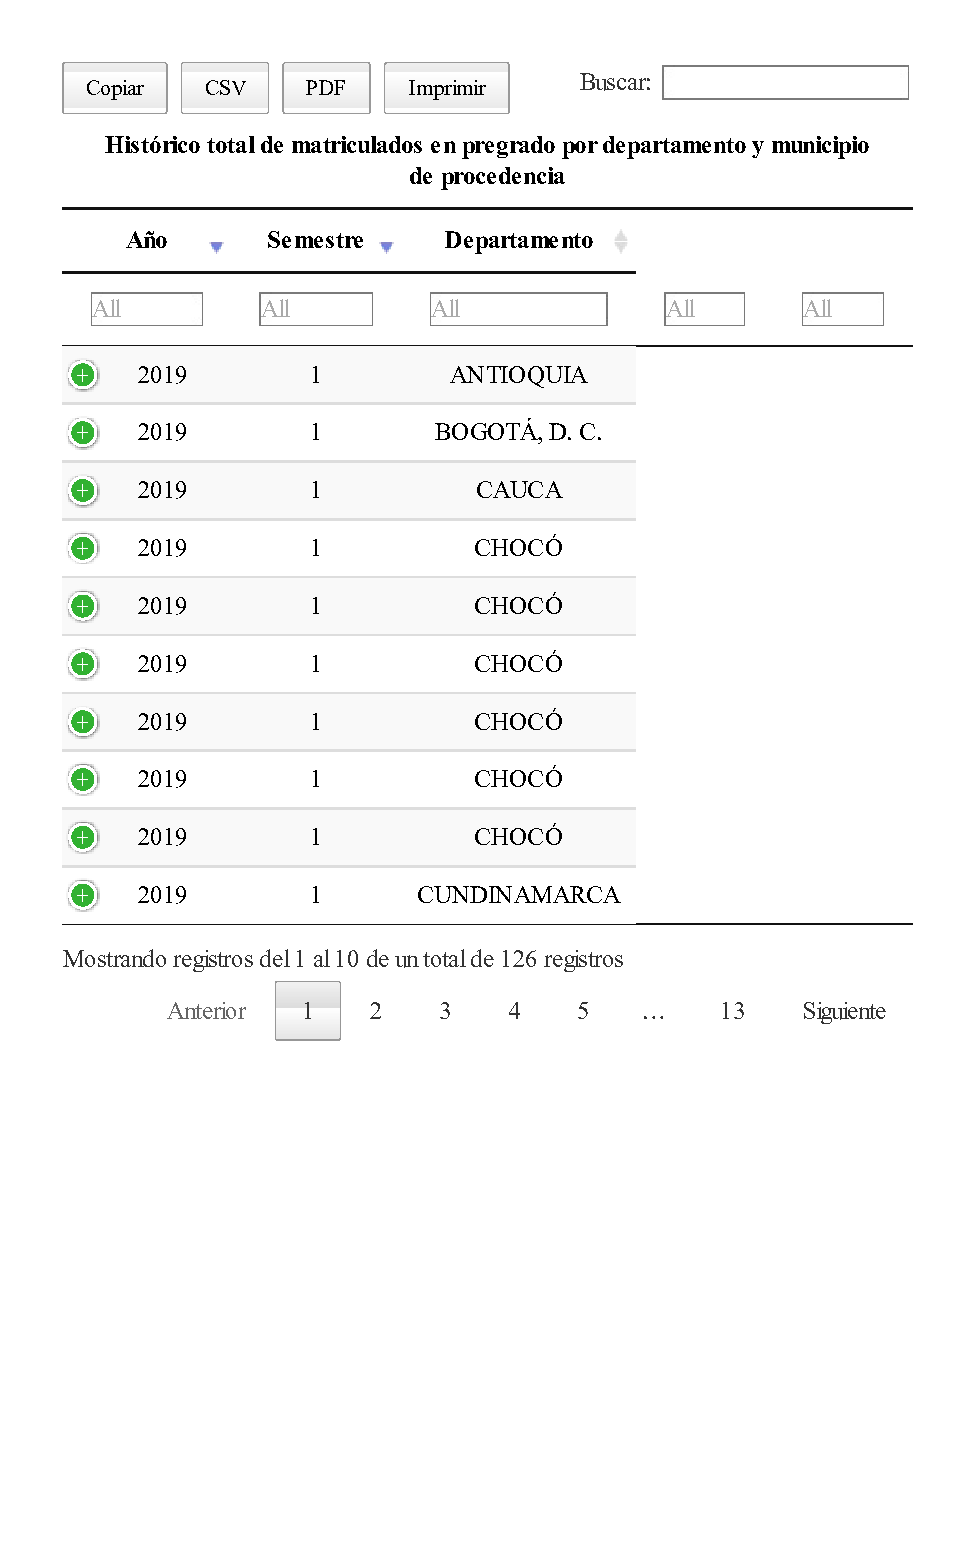
\includegraphics{BoletinTumaco_files/figure-latex/F12MatPre-1.pdf}
\caption{\label{fig:F12MatPre}Fuente: Dirección Nacional de Planeación y Estadística con base en información de la Dirección Nacional Información Académica}
\end{figure}

\hypertarget{programas-acaduxe9micos-de-pregrado-1}{%
\subsubsection{Programas académicos de pregrado}\label{programas-acaduxe9micos-de-pregrado-1}}

A continuación, la Tabla \ref{fig:F13MatPre} presenta el acumulado histórico de matriculados en pregrado, en la \textbf{Sede Tumaco}, por años, semestres, sedes andinas, facultades y programas académicos cursados.

\begin{figure}
\centering
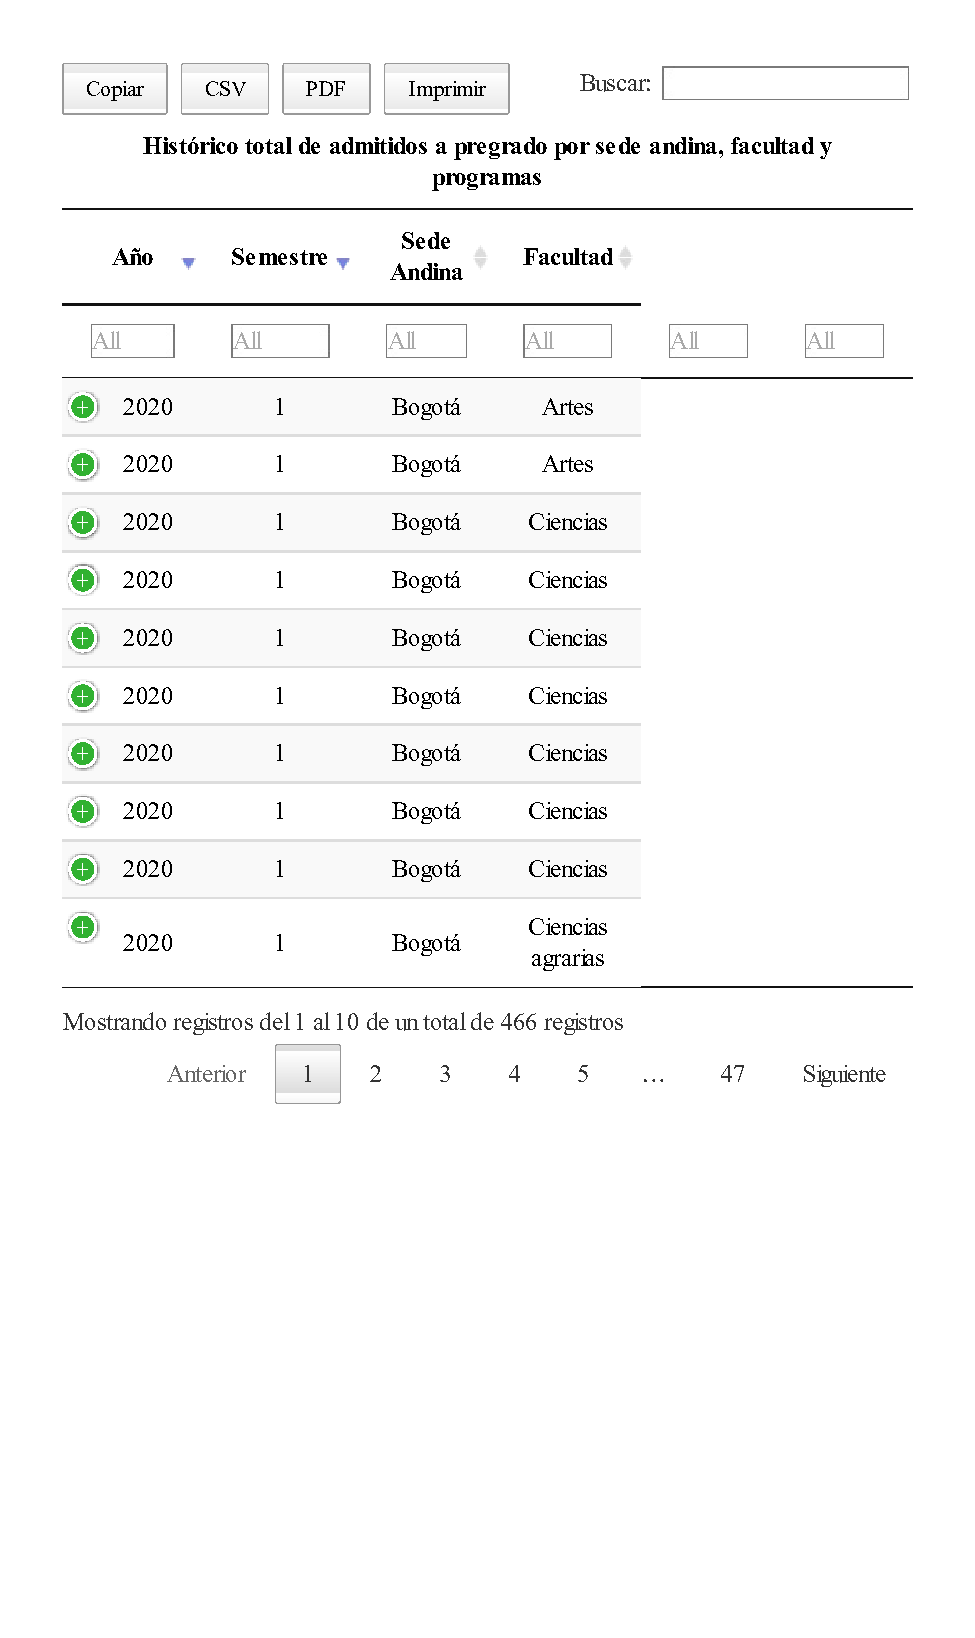
\includegraphics{BoletinTumaco_files/figure-latex/F13MatPre-1.pdf}
\caption{\label{fig:F13MatPre}Fuente: Dirección Nacional de Planeación y Estadística con base en información de la Dirección Nacional Información Académica}
\end{figure}

\hypertarget{MatPreIni}{%
\section{Matriculados en pregrado - Etapa Inicial}\label{MatPreIni}}

A continuación, se presenta la información oficial del total de estudiantes matricualdos en pregrado en la Universidad y que han sido admitidos a través de la \textbf{Sede Tumaco}. Incluye los estudiantes de pregrado que se encuentran en la \textbf{etapa inicial} del proceso de formación; es decir, \textbf{ubicados de manera presencial} en la Sede Tumaco. En específico, se presenta la evolución histórica de los matriculados en pregrado en etapa inicial desde diferentes perspectivas: general, sedes andinas, sexo, grupos de edad, estrato socioeconómico, departamentos y municipios de residencia y programas académicos de pregrado en los que estos se encuentran matriculados. Para cada una de las variables analizadas se presenta la evolución histórica (\emph{serie de tiempo}) así como el comportamiento actual (\emph{estado actual}) derivado de las últimas mediciones disponibles.

\hypertarget{evoluciuxf3n-histuxf3rica-3}{%
\subsection{Evolución histórica}\label{evoluciuxf3n-histuxf3rica-3}}

A continuación, la Figura \ref{fig:F1MatPreFI}, presenta la evolución histórica -\emph{desde el periodo 20151}-, del total de matriculados en pregrado -etapa inicial- en la \textbf{Sede Tumaco}.

\begin{figure}
\centering
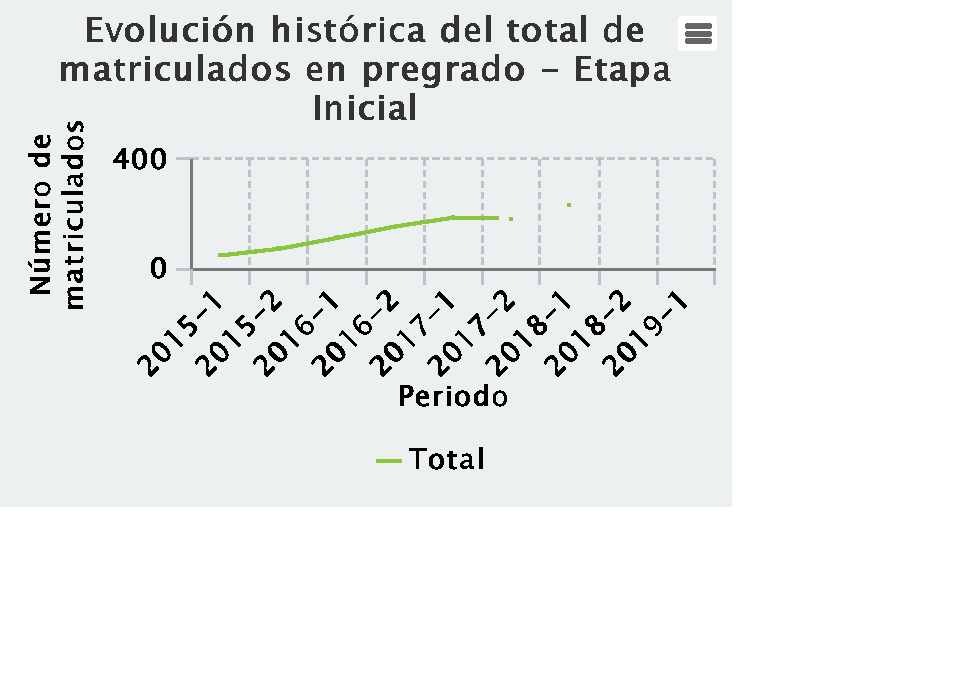
\includegraphics{BoletinTumaco_files/figure-latex/F1MatPreFI-1.pdf}
\caption{\label{fig:F1MatPreFI}Fuente: Dirección Nacional de Planeación y Estadística con base en información de la Dirección Nacional Información Académica}
\end{figure}

\hypertarget{informaciuxf3n-por-sede-andina-1}{%
\subsection{Información por sede andina}\label{informaciuxf3n-por-sede-andina-1}}

A continuación, las figuras \ref{fig:F2MatPreFI} y \ref{fig:F3MatPreFI} presentan, respectivamente, la evolución histórica y el comportamiento actual del total de estudiantes matriculados de pregrado - etapa inicial- en la \textbf{Sede Tumaco} según la sede andina en la que estos cursarán sus estudios de pregrado en la etapa de movilidad.

\begin{figure}
\centering
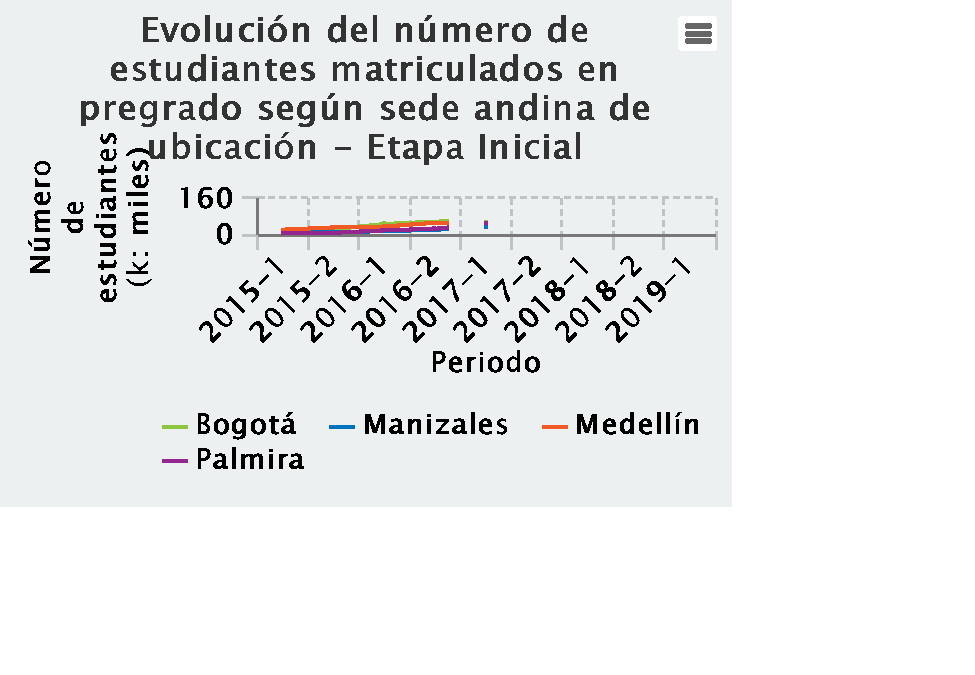
\includegraphics{BoletinTumaco_files/figure-latex/F2MatPreFI-1.pdf}
\caption{\label{fig:F2MatPreFI}Fuente: Dirección Nacional de Planeación y Estadística con base en información de la Dirección Nacional Información Académica}
\end{figure}

\begin{figure}
\centering
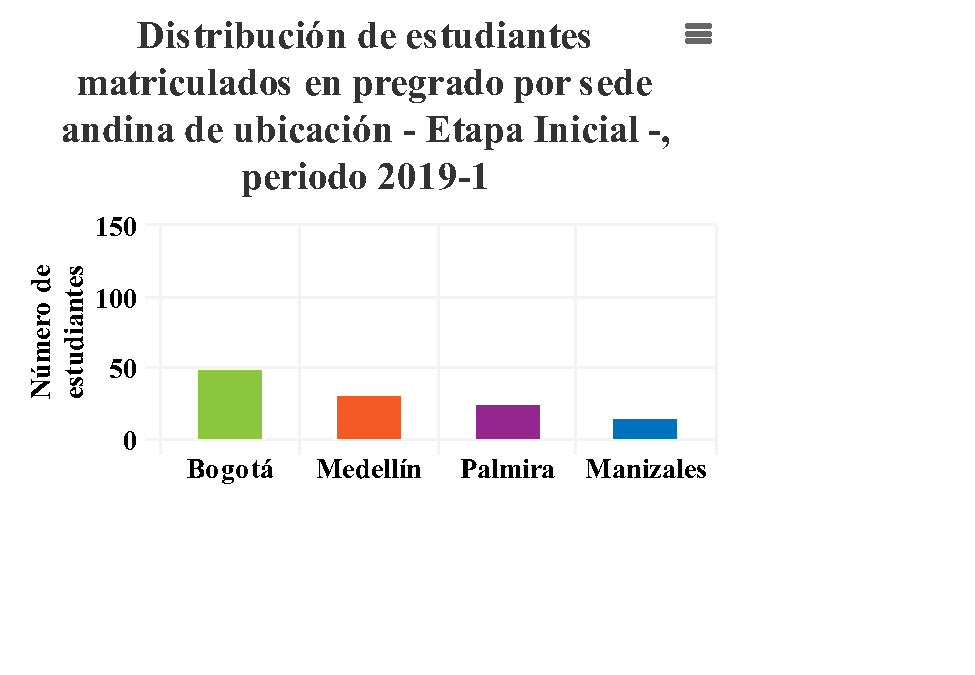
\includegraphics{BoletinTumaco_files/figure-latex/F3MatPreFI-1.pdf}
\caption{\label{fig:F3MatPreFI}Fuente: Dirección Nacional de Planeación y Estadística con base en información de la Dirección Nacional Información Académica}
\end{figure}

\hypertarget{informaciuxf3n-por-sexo-3}{%
\subsection{Información por sexo}\label{informaciuxf3n-por-sexo-3}}

A continuación, las figuras \ref{fig:F4MatPreFI} y \ref{fig:F5MatPreFI} presentan, respectivamente, la evolución histórica y el comportamiento actual del total de matriculados en pregrado -etapa inicial- en la \textbf{Sede Tumaco} según el sexo biológico.

\begin{figure}
\centering
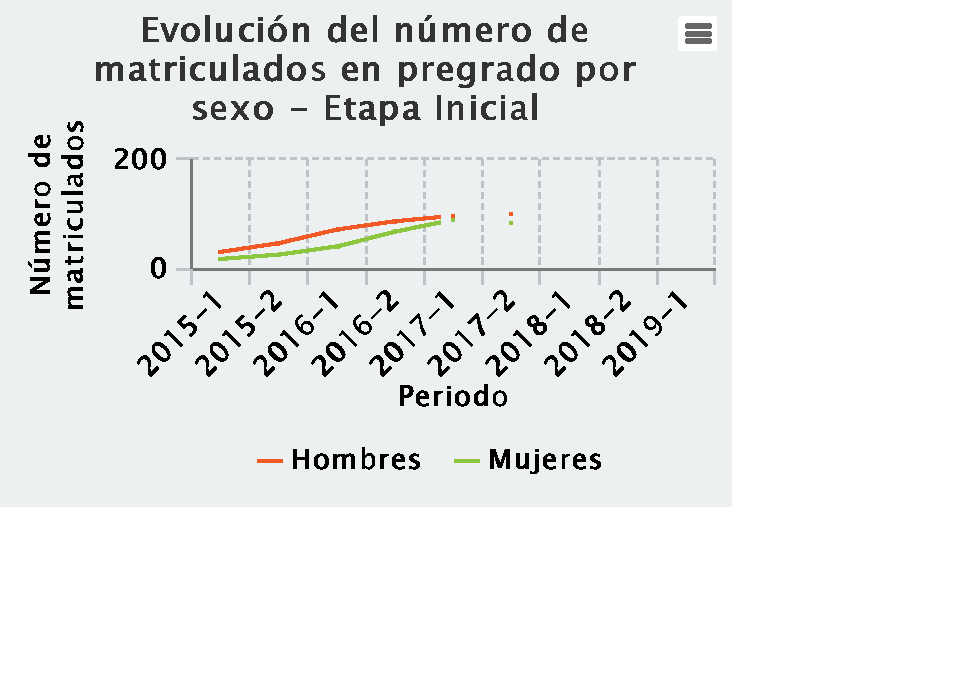
\includegraphics{BoletinTumaco_files/figure-latex/F4MatPreFI-1.pdf}
\caption{\label{fig:F4MatPreFI}Fuente: Dirección Nacional de Planeación y Estadística con base en información de la Dirección Nacional Información Académica}
\end{figure}

\begin{figure}
\centering
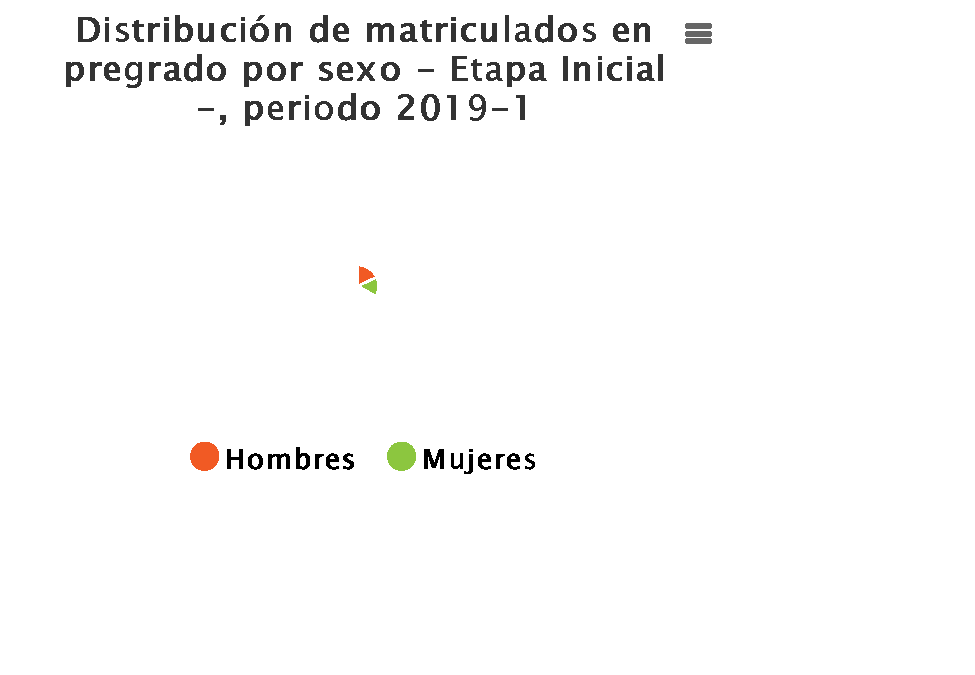
\includegraphics{BoletinTumaco_files/figure-latex/F5MatPreFI-1.pdf}
\caption{\label{fig:F5MatPreFI}Fuente: Dirección Nacional de Planeación y Estadística con base en información de la Dirección Nacional Información Académica}
\end{figure}

\hypertarget{informaciuxf3n-por-edad-3}{%
\subsection{Información por edad}\label{informaciuxf3n-por-edad-3}}

A continuación, las figuras \ref{fig:F6MatPreFI} y \ref{fig:F7MatPreFI} presentan, respectivamente, la evolución histórica y el comportamiento actual del total de estudiantes matriculados en pregrado -etapa inicial- de la \textbf{Sede Tumaco} según grupos de edad.

\begin{figure}
\centering
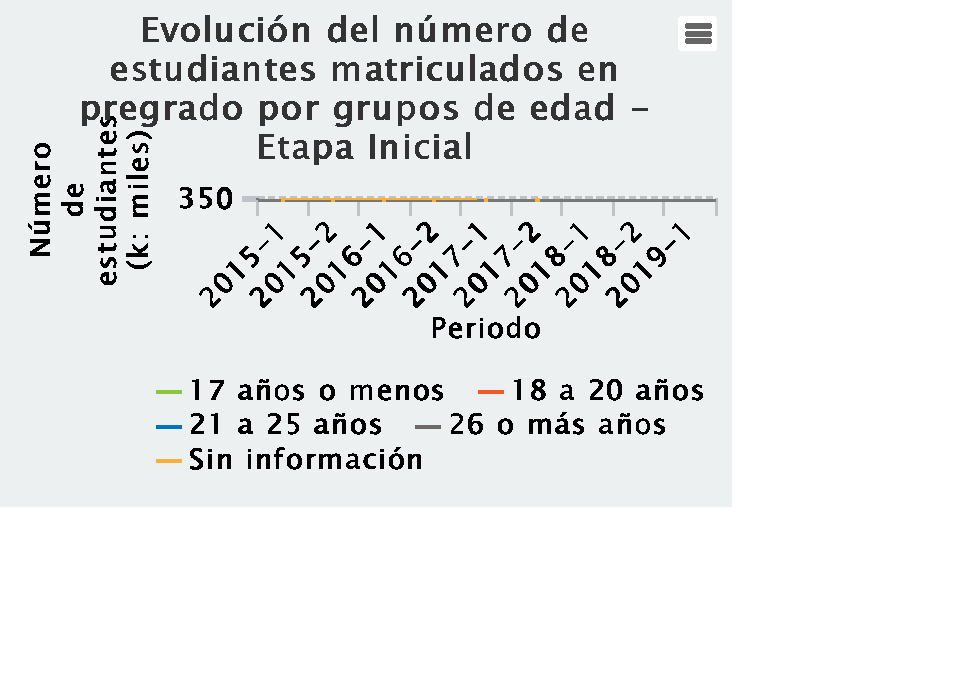
\includegraphics{BoletinTumaco_files/figure-latex/F6MatPreFI-1.pdf}
\caption{\label{fig:F6MatPreFI}Fuente: Dirección Nacional de Planeación y Estadística con base en información de la Dirección Nacional Información Académica}
\end{figure}

\begin{figure}
\centering
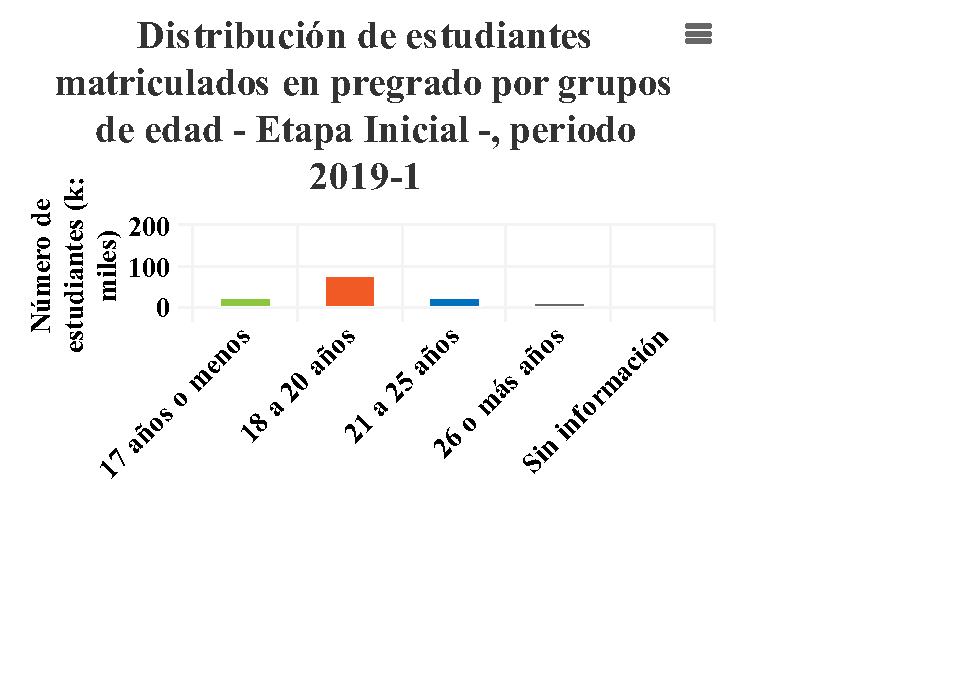
\includegraphics{BoletinTumaco_files/figure-latex/F7MatPreFI-1.pdf}
\caption{\label{fig:F7MatPreFI}Fuente: Dirección Nacional de Planeación y Estadística con base en información de la Dirección Nacional Información Académica}
\end{figure}

\hypertarget{informaciuxf3n-por-estrato-1}{%
\subsection{Información por estrato}\label{informaciuxf3n-por-estrato-1}}

A continuación, las figuras \ref{fig:F8MatPreFI} y \ref{fig:F9MatPreFI} presentan, respectivamente, la evolución histórica y el comportamiento actual del total de estudiantes matriculados en pregrado -etapa inicial- en la \textbf{Sede Tumaco} según el estrato socioeconómico.

\begin{figure}
\centering
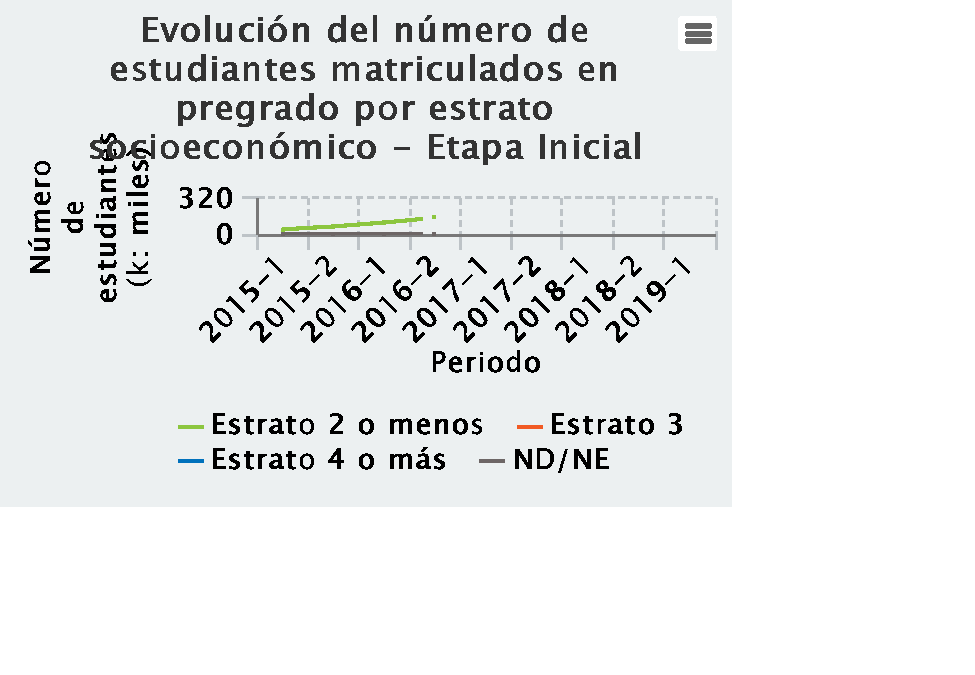
\includegraphics{BoletinTumaco_files/figure-latex/F8MatPreFI-1.pdf}
\caption{\label{fig:F8MatPreFI}Fuente: Dirección Nacional de Planeación y Estadística con base en información de la Dirección Nacional Información Académica}
\end{figure}

\begin{figure}
\centering
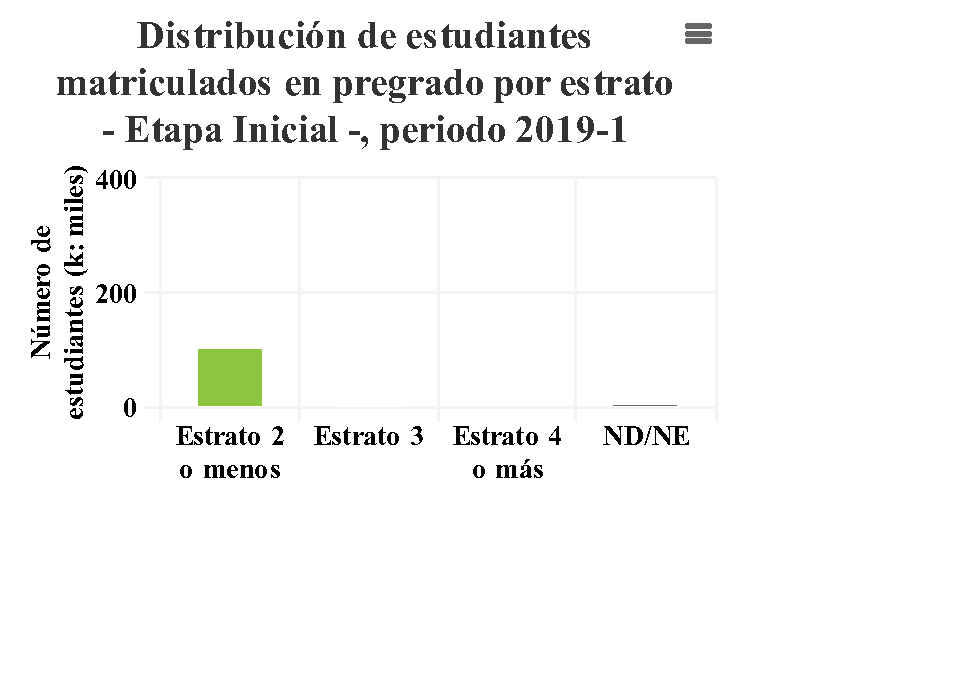
\includegraphics{BoletinTumaco_files/figure-latex/F9MatPreFI-1.pdf}
\caption{\label{fig:F9MatPreFI}Fuente: Dirección Nacional de Planeación y Estadística con base en información de la Dirección Nacional Información Académica}
\end{figure}

\hypertarget{tablas-cifras-agregadas-3}{%
\subsection{Tablas cifras agregadas}\label{tablas-cifras-agregadas-3}}

A continuación se presentan, a través de tablas, los agregados/consolidados históricos del total de matriculados en pregrado -etapa inicial- de la \textbf{Sede Tumaco} por departamentos y municipios de procedencia así como los programas académicos de pregrado que estos cursan en las sedes andinas de la Universidad (Bogotá, Medellín, Manizales o Palmira).

Los interesados en \emph{imprimir}, \emph{copiar} o \emph{descargar} estas cifras, pueden hacerlo a través de las múltiples opciones que se ofrecen en la parte superior izquierda de cada una de las tablas (Copiar, CSV, Excel, PDF e Imprimir). Así mismo, estas tablas permiten filtrar los resultados por aquellas variables de interés.

\hypertarget{departamentos-y-municipios-de-procedencia-2}{%
\subsubsection{Departamentos y municipios de procedencia}\label{departamentos-y-municipios-de-procedencia-2}}

A continuación, la Tabla \ref{fig:F10MatPreFI} presenta los acumulados \textbf{históricos}, por \textbf{años y semestres}, en la \textbf{Sede Tumaco}, de los matriculados en pregrado -etapa inicial- por departamentos y municipios de procedencia.

\begin{figure}
\centering
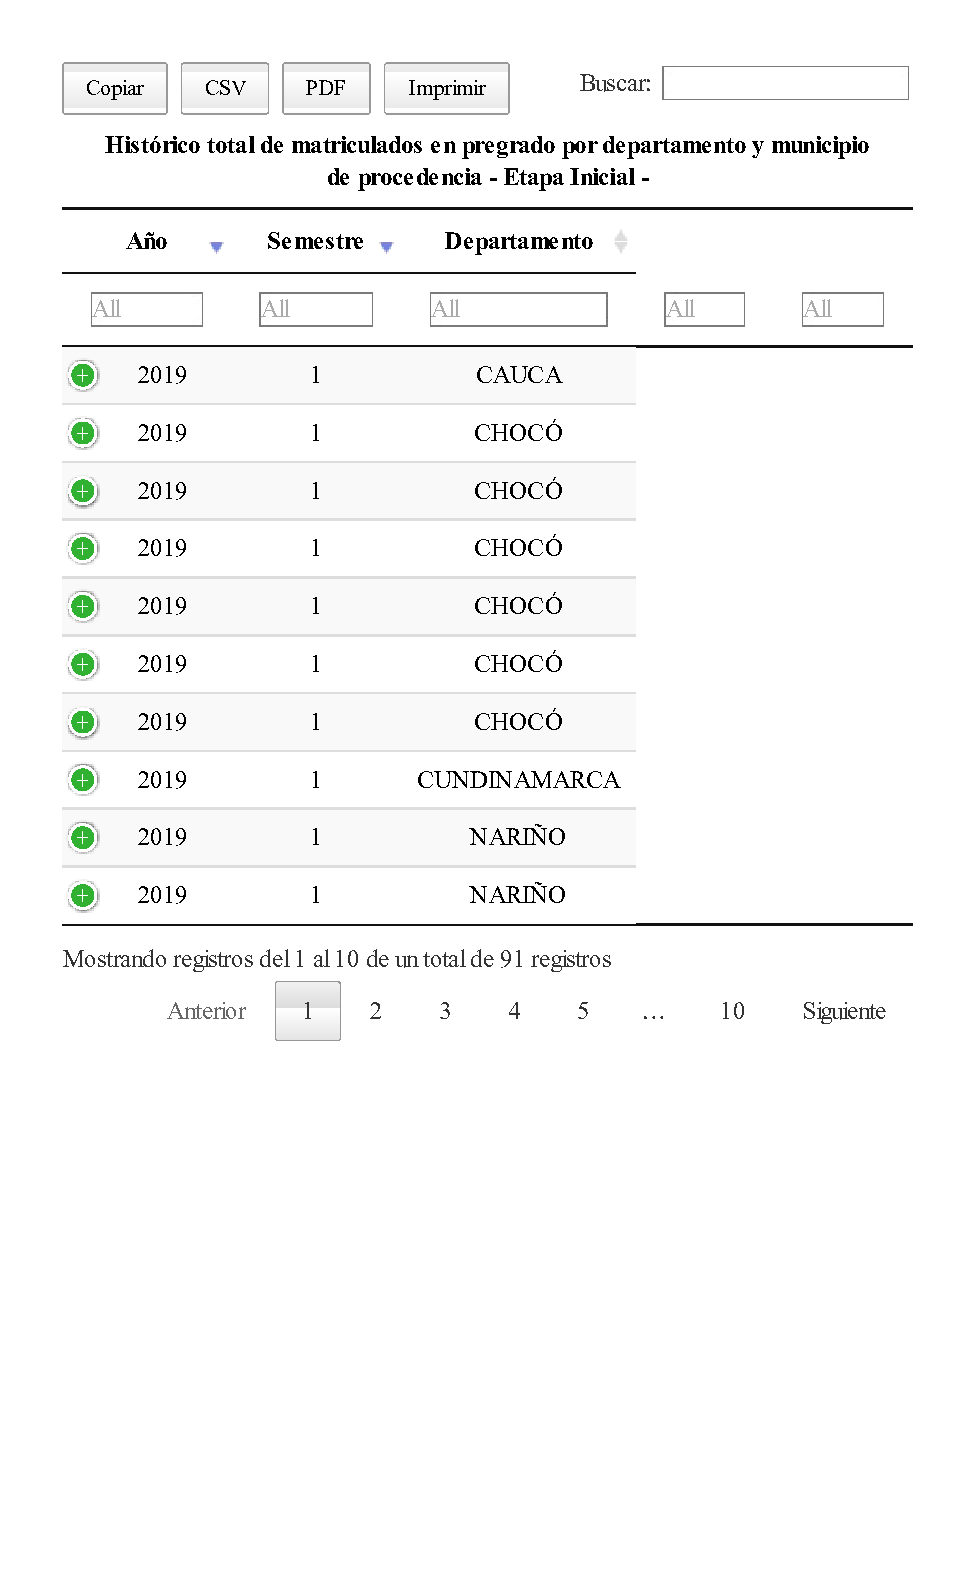
\includegraphics{BoletinTumaco_files/figure-latex/F10MatPreFI-1.pdf}
\caption{\label{fig:F10MatPreFI}Fuente: Dirección Nacional de Planeación y Estadística con base en información de la Dirección Nacional Información Académica}
\end{figure}

\hypertarget{programas-acaduxe9micos-de-pregrado-2}{%
\subsubsection{Programas académicos de pregrado}\label{programas-acaduxe9micos-de-pregrado-2}}

A continuación, la Tabla \ref{fig:F11MatPreFI} presenta el acumulado histórico de matriculados en pregrado -etapa inicial-, en la \textbf{Sede Tumaco}, por años, semestres, sedes andinas, facultades y programas académicos cursados.

\begin{figure}
\centering
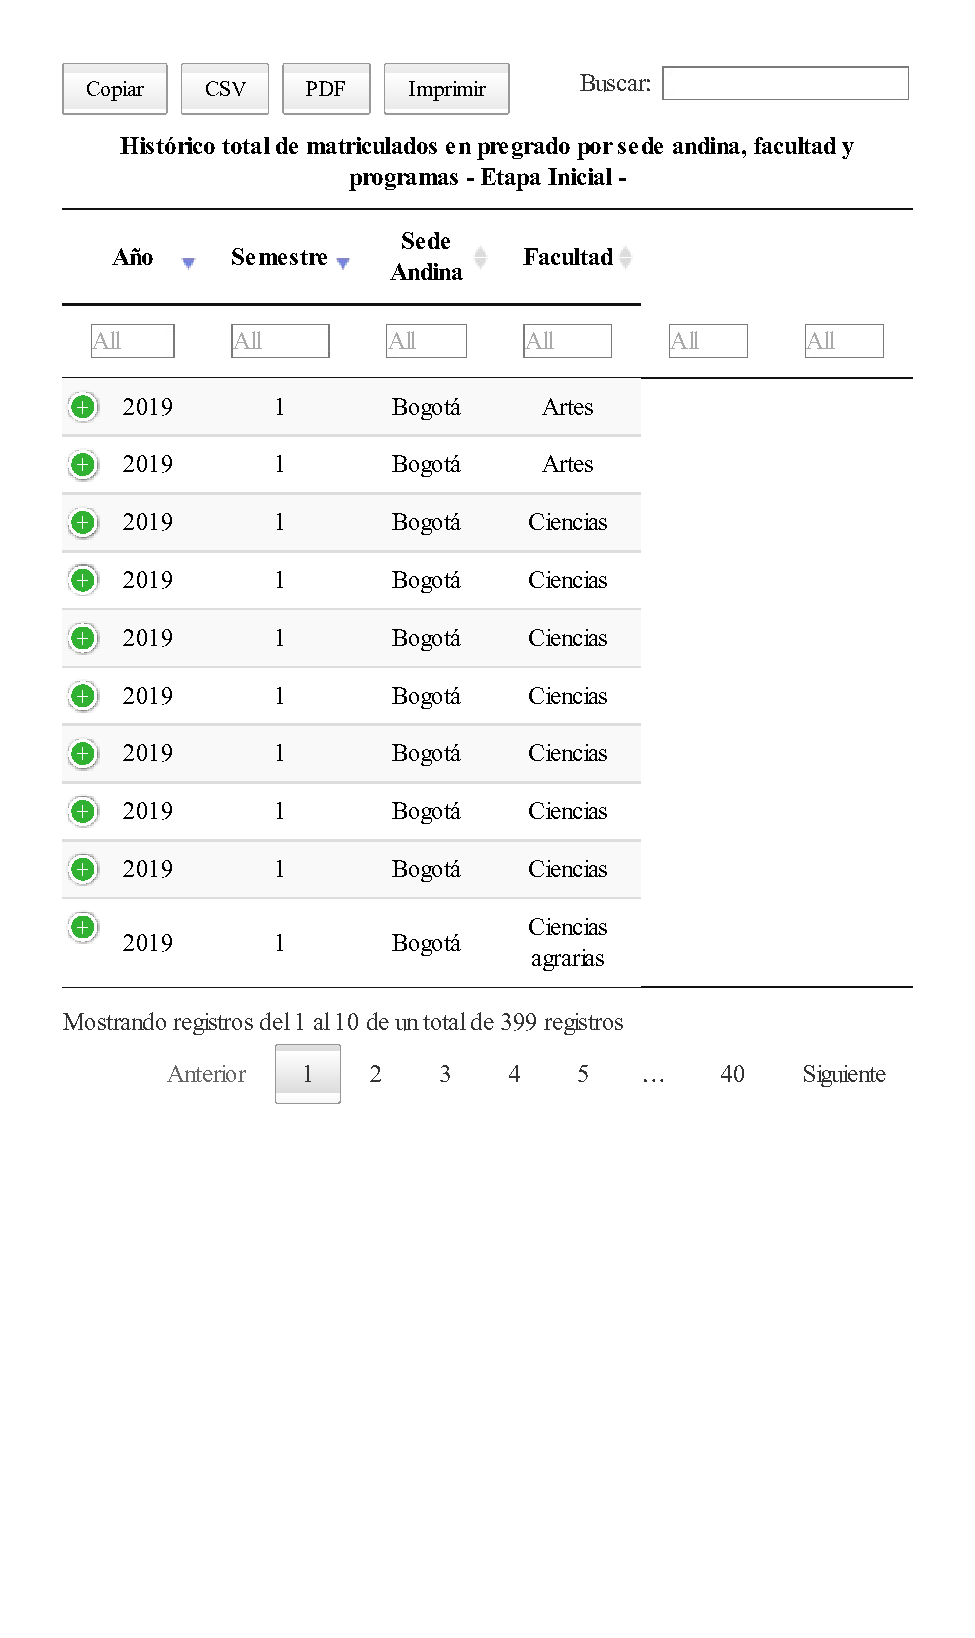
\includegraphics{BoletinTumaco_files/figure-latex/F11MatPreFI-1.pdf}
\caption{\label{fig:F11MatPreFI}Fuente: Dirección Nacional de Planeación y Estadística con base en información de la Dirección Nacional Información Académica}
\end{figure}

\hypertarget{MatPreMov}{%
\section{Matriculados en pregrado - Etapa Movilidad}\label{MatPreMov}}

A continuación, se presenta la información oficial del total de estudiantes matricualdos en pregrado en la Universidad y que han sido admitidos a través de la \textbf{Sede Tumaco}. Incluye los estudiantes de pregrado que se encuentran en la \textbf{etapa de movilidad} del proceso de formación; es decir, \textbf{ubicados de manera presencial} en las sedes andinas de la Universidad (Bogotá, Medellín, Manizales o Palmira). En específico, se presenta la evolución histórica de los matriculados en pregrado en etapa de movilidad desde diferentes perspectivas: general, sedes andinas de ubicación, sexo, grupos de edad, estrato socioeconómico, departamentos y municipios de residencia y programas académicos de pregrado en los que estos se encuentran matriculados. Para cada una de las variables analizadas se presenta la evolución histórica (\emph{serie de tiempo}) así como el comportamiento actual (\emph{estado actual}) derivado de las últimas mediciones disponibles.

\hypertarget{evoluciuxf3n-histuxf3rica-4}{%
\subsection{Evolución histórica}\label{evoluciuxf3n-histuxf3rica-4}}

A continuación, la Figura \ref{fig:F1MatPreFM}, presenta la evolución histórica -\emph{desde el periodo 20152}-, del total de matriculados en pregrado -etapa de movilidad- en la \textbf{Sede Tumaco}.

\begin{figure}
\centering
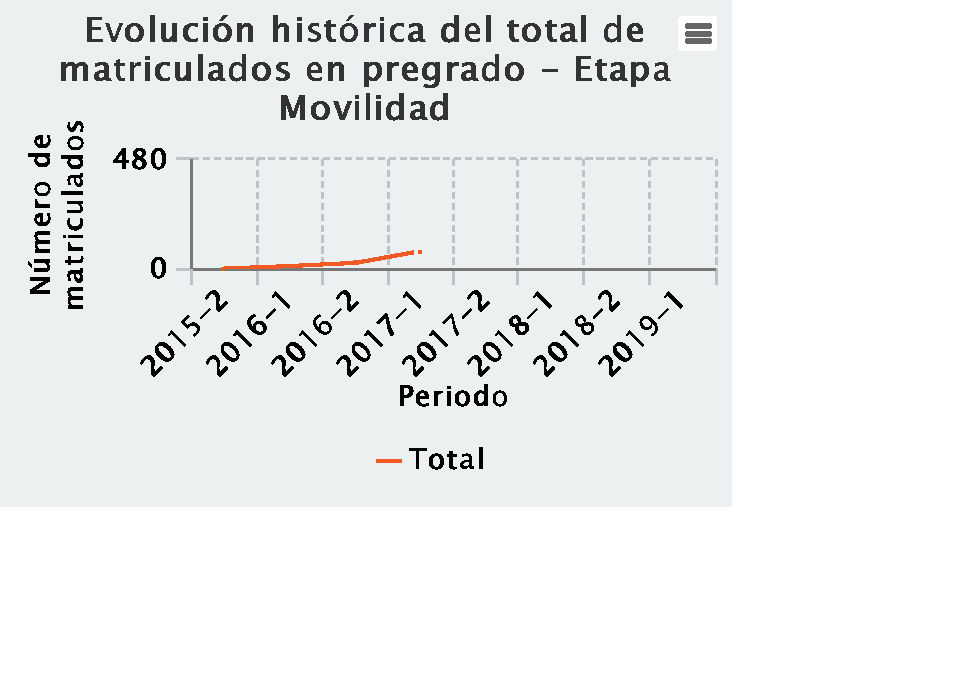
\includegraphics{BoletinTumaco_files/figure-latex/F1MatPreFM-1.pdf}
\caption{\label{fig:F1MatPreFM}Fuente: Dirección Nacional de Planeación y Estadística con base en información de la Dirección Nacional Información Académica}
\end{figure}

\hypertarget{informaciuxf3n-por-sede-andina-2}{%
\subsection{Información por sede andina}\label{informaciuxf3n-por-sede-andina-2}}

A continuación, las figuras \ref{fig:F2MatPreFM} y \ref{fig:F3MatPreFM} presentan, respectivamente, la evolución histórica y el comportamiento actual del total de estudiantes matriculados de pregrado - etapa de movilidad- en la \textbf{Sede Tumaco} según la sede andina en la que estos se encuentran cursando sus estudios de pregrado en la etapa de movilidad.

\begin{figure}
\centering
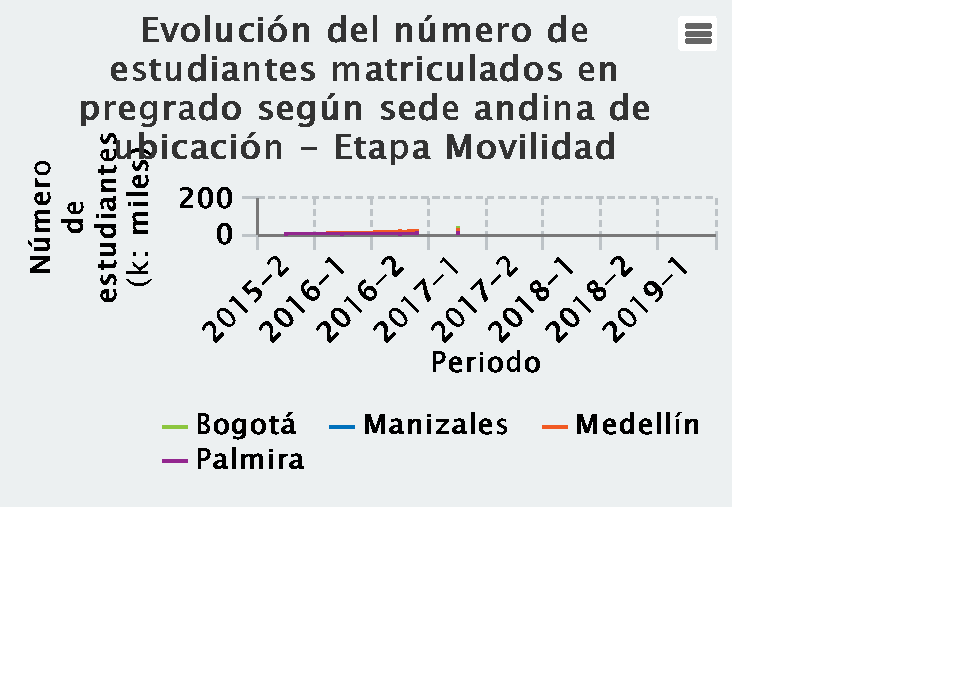
\includegraphics{BoletinTumaco_files/figure-latex/F2MatPreFM-1.pdf}
\caption{\label{fig:F2MatPreFM}Fuente: Dirección Nacional de Planeación y Estadística con base en información de la Dirección Nacional Información Académica}
\end{figure}

\begin{figure}
\centering
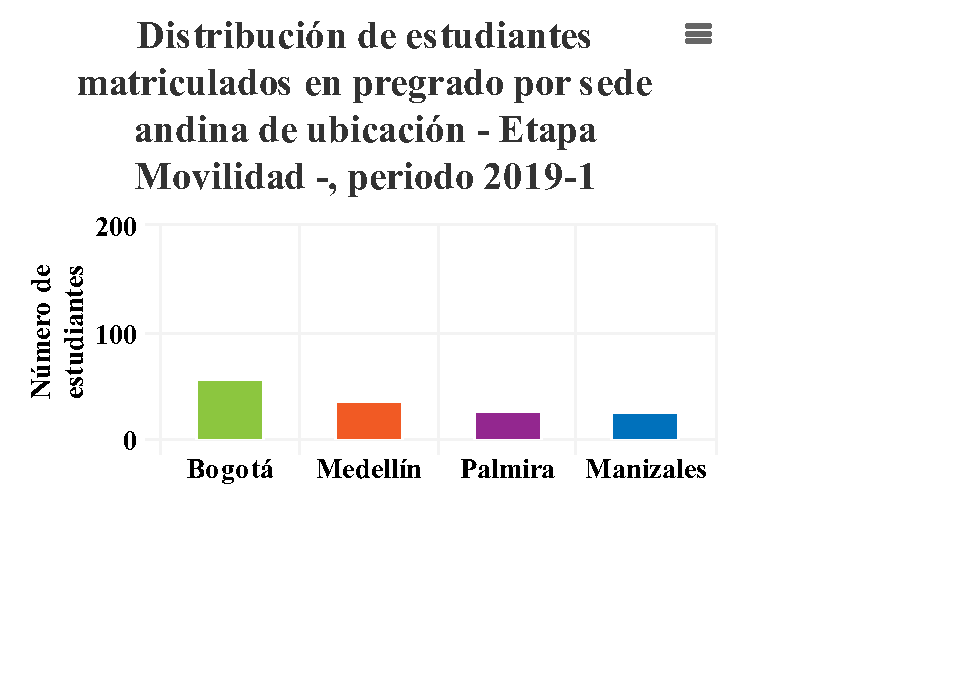
\includegraphics{BoletinTumaco_files/figure-latex/F3MatPreFM-1.pdf}
\caption{\label{fig:F3MatPreFM}Fuente: Dirección Nacional de Planeación y Estadística con base en información de la Dirección Nacional Información Académica}
\end{figure}

\hypertarget{informaciuxf3n-por-sexo-4}{%
\subsection{Información por sexo}\label{informaciuxf3n-por-sexo-4}}

A continuación, las figuras \ref{fig:F4MatPreFM} y \ref{fig:F5MatPreFM} presentan, respectivamente, la evolución histórica y el comportamiento actual del total de matriculados en pregrado -etapa de movilidad- en la \textbf{Sede Tumaco} según el sexo biológico.

\begin{figure}
\centering
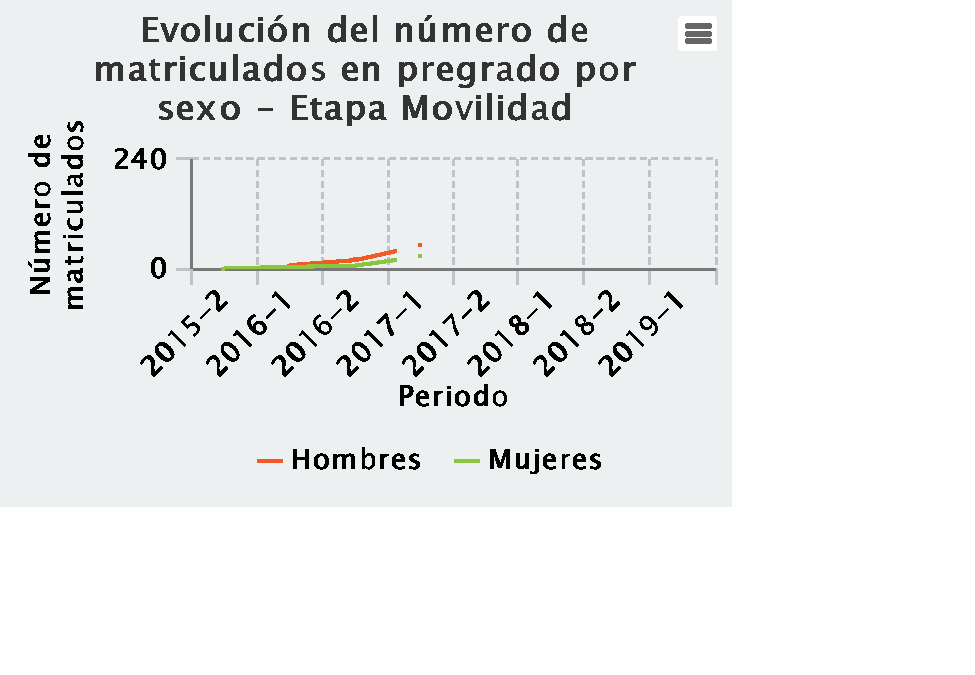
\includegraphics{BoletinTumaco_files/figure-latex/F4MatPreFM-1.pdf}
\caption{\label{fig:F4MatPreFM}Fuente: Dirección Nacional de Planeación y Estadística con base en información de la Dirección Nacional Información Académica}
\end{figure}

\begin{figure}
\centering
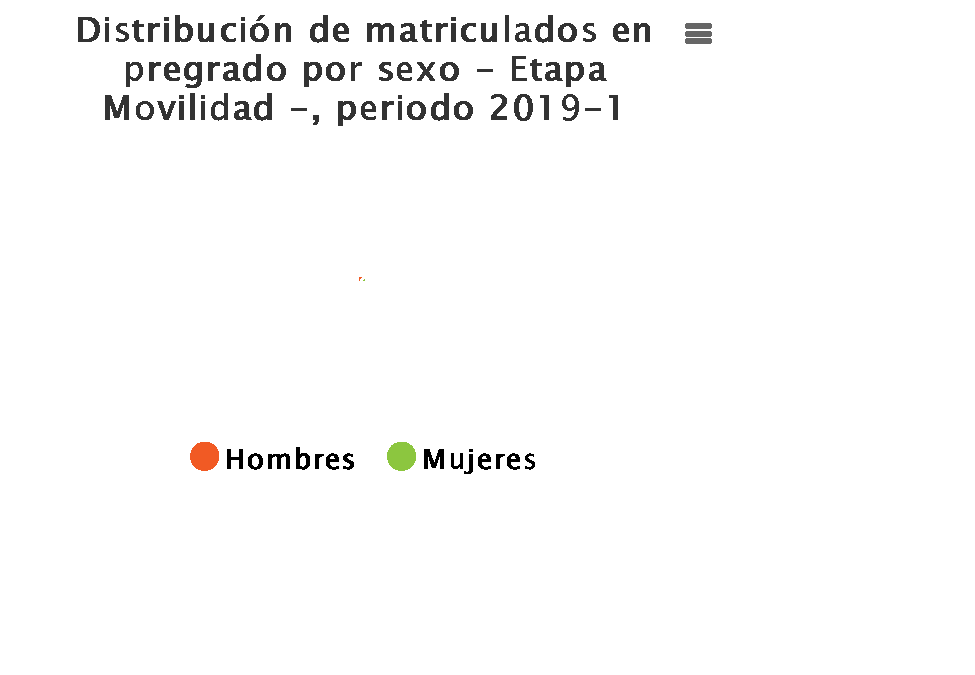
\includegraphics{BoletinTumaco_files/figure-latex/F5MatPreFM-1.pdf}
\caption{\label{fig:F5MatPreFM}Fuente: Dirección Nacional de Planeación y Estadística con base en información de la Dirección Nacional Información Académica}
\end{figure}

\hypertarget{informaciuxf3n-por-edad-4}{%
\subsection{Información por edad}\label{informaciuxf3n-por-edad-4}}

A continuación, las figuras \ref{fig:F6MatPreFM} y \ref{fig:F7MatPreFM} presentan, respectivamente, la evolución histórica y el comportamiento actual del total de estudiantes matriculados en pregrado -etapa de movilidad- de la \textbf{Sede Tumaco} según grupos de edad.

\begin{figure}
\centering
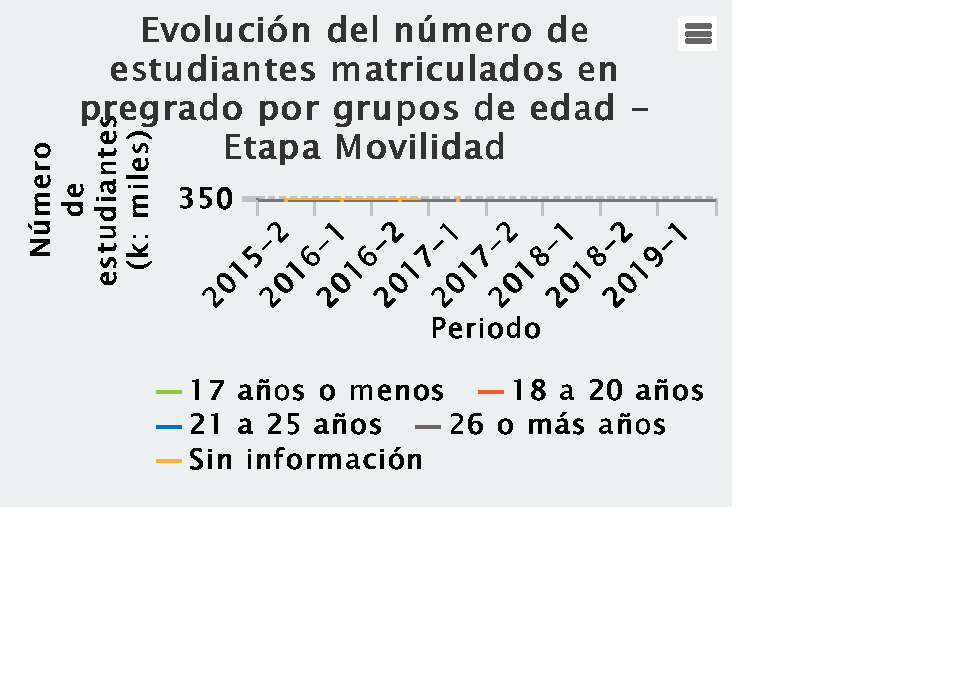
\includegraphics{BoletinTumaco_files/figure-latex/F6MatPreFM-1.pdf}
\caption{\label{fig:F6MatPreFM}Fuente: Dirección Nacional de Planeación y Estadística con base en información de la Dirección Nacional Información Académica}
\end{figure}

\begin{figure}
\centering
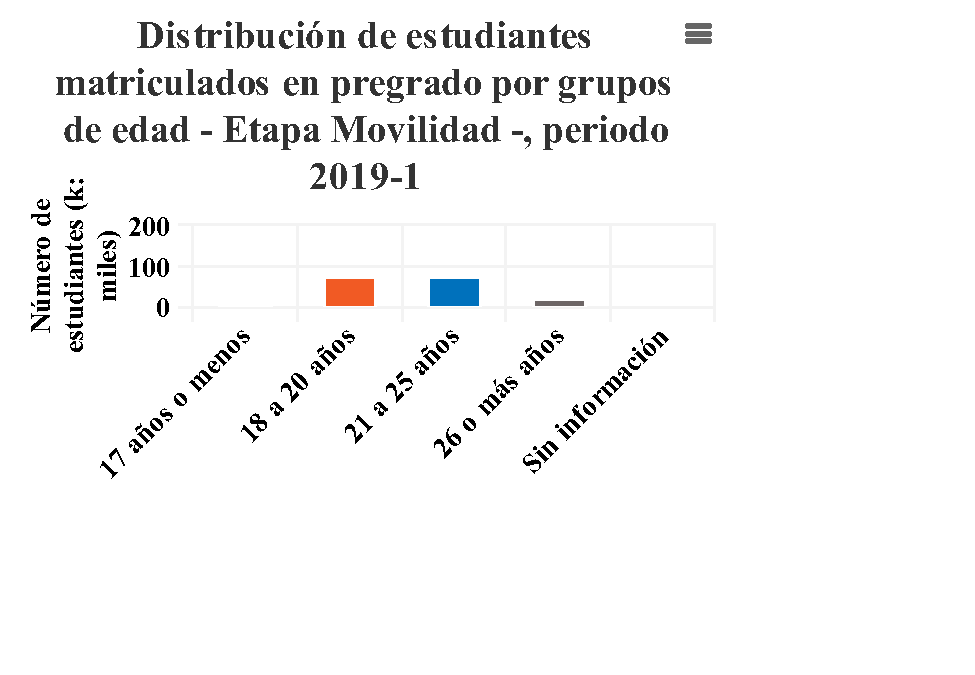
\includegraphics{BoletinTumaco_files/figure-latex/F7MatPreFM-1.pdf}
\caption{\label{fig:F7MatPreFM}Fuente: Dirección Nacional de Planeación y Estadística con base en información de la Dirección Nacional Información Académica}
\end{figure}

\hypertarget{informaciuxf3n-por-estrato-2}{%
\subsection{Información por estrato}\label{informaciuxf3n-por-estrato-2}}

A continuación, las figuras \ref{fig:F8MatPreFM} y \ref{fig:F9MatPreFM} presentan, respectivamente, la evolución histórica y el comportamiento actual del total de estudiantes matriculados en pregrado -etapa de movilidad- en la \textbf{Sede Tumaco} según el estrato socioeconómico.

\begin{figure}
\centering
\includegraphics{BoletinTumaco_files/figure-latex/F8MatPreFM-1.pdf}
\caption{\label{fig:F8MatPreFM}Fuente: Dirección Nacional de Planeación y Estadística con base en información de la Dirección Nacional Información Académica}
\end{figure}

\begin{figure}
\centering
\includegraphics{BoletinTumaco_files/figure-latex/F9MatPreFM-1.pdf}
\caption{\label{fig:F9MatPreFM}Fuente: Dirección Nacional de Planeación y Estadística con base en información de la Dirección Nacional Información Académica}
\end{figure}

\hypertarget{tablas-cifras-agregadas-4}{%
\subsection{Tablas cifras agregadas}\label{tablas-cifras-agregadas-4}}

A continuación se presentan, a través de tablas, los agregados/consolidados históricos del total de matriculados en pregrado -etapa de movilidad- de la \textbf{Sede Tumaco} por departamentos y municipios de procedencia así como los programas académicos de pregrado que estos cursan en las sedes andinas de la Universidad (Bogotá, Medellín, Manizales y Palmira).

Los interesados en \emph{imprimir}, \emph{copiar} o \emph{descargar} estas cifras, pueden hacerlo a través de las múltiples opciones que se ofrecen en la parte superior izquierda de cada una de las tablas (Copiar, CSV, Excel, PDF e Imprimir). Así mismo, estas tablas permiten filtrar los resultados por aquellas variables de interés.

\hypertarget{departamentos-y-municipios-de-procedencia-3}{%
\subsubsection{Departamentos y municipios de procedencia}\label{departamentos-y-municipios-de-procedencia-3}}

A continuación, la Tabla \ref{fig:F10MatPreFM} presenta los acumulados \textbf{históricos}, por \textbf{años y semestres}, en la \textbf{Sede Tumaco}, de los matriculados en pregrado -etapa de movilidad- por departamentos y municipios de procedencia.

\begin{figure}
\centering
\includegraphics{BoletinTumaco_files/figure-latex/F10MatPreFM-1.pdf}
\caption{\label{fig:F10MatPreFM}Fuente: Dirección Nacional de Planeación y Estadística con base en información de la Dirección Nacional Información Académica}
\end{figure}

\hypertarget{programas-acaduxe9micos-de-pregrado-3}{%
\subsubsection{Programas académicos de pregrado}\label{programas-acaduxe9micos-de-pregrado-3}}

A continuación, la Tabla \ref{fig:F11MatPreFM} presenta el acumulado histórico de matriculados en pregrado -etapa de movilidad-, en la \textbf{Sede Tumaco}, por años, semestres, sedes andinas, facultades y programas académicos cursados.

\begin{figure}
\centering
\includegraphics{BoletinTumaco_files/figure-latex/F11MatPreFM-1.pdf}
\caption{\label{fig:F11MatPreFM}Fuente: Dirección Nacional de Planeación y Estadística con base en información de la Dirección Nacional Información Académica}
\end{figure}

\hypertarget{Grad}{%
\chapter{Graduados}\label{Grad}}

La \textbf{Sede Tumaco} de la Universidad Nacional de Colombia, dada la \textbf{reciente apertura} para la formación de estudiantes en programas académicos de pregrado, \textbf{aún no cuenta con estudiantes graduados en este nivel de formación}. Se espera que en el próximos dos años se presenten los primeros graduados.

\hypertarget{Doc}{%
\chapter{Docentes}\label{Doc}}

La Sede Tumaco, a la fecha, \textbf{no cuenta con docentes de carrera} adscritos de manera formal a esta sede. En esta sede, el proceso de formación de los estudiantes se da a través de varias modalidades de apoyo académico entre las que se destacan: \ldots.

\hypertarget{DocCar}{%
\section{Docentes de carrera}\label{DocCar}}

La Sede Tumaco, a la fecha, \textbf{no cuenta con docentes de carrera} adscritos de manera formal a esta sede.

\hypertarget{DocPEAMA}{%
\section{Docentes PEAMA}\label{DocPEAMA}}

\hypertarget{DocApo}{%
\section{Profesionales de apoyo PEAMA}\label{DocApo}}

\hypertarget{Admi}{%
\chapter{Administrativos}\label{Admi}}

Este capítulo presenta el consolidado de las principales características asociadas a la información estadística oficial de los administrativos de carrera adscritos a la Sede Tumaco de la Universidad Nacional de Colombia así como la información estadística del personal adicional que apoya las labores administrativas en esta sede y que se encuentran vinculados a través de contratos de prestación de servicios (contratistas).

A continuación, se presenta una breve descripción de las secciones que hacen parte de este capítulo así como la ubicación del sitio web en donde se presentan las definiciones, los estándares y las codificaciones/clasificaciones que hacen parte de la información acá contenida (\emph{metadatos}) y cuya exploración y lectura, sin duda, facilitará el entendimiento de las cifras asociadas, principalmente, a la población de administrativos de carrera en esta sede de la Universidad.

\textbf{Secciones}

\begin{itemize}
\item
  \protect\hyperlink{AdmCar}{Administrativos de carrera}: contiene la información oficial del total de funcionarios administrativos de carrera adscritos a la Sede Tumaco de la Universidad Nacional de Colombia y que fueron vinculados mediante concurso público.
\item
  \protect\hyperlink{Contrat}{Contratistas}: contiene la información oficial del total de \ldots..
\end{itemize}

\textbf{Metadatos}

La construcción de las cifras oficiales de administrativos de carrera en la Sede Tumaco, las definiciones que hacen parte de esta categoría así como las codificaciones y clasificaciones aquí empleadas se encuentran contenidas en la sección \textbf{Administrativos} del capítulo de \emph{Metadatos} de las cifras oficiales generales que hacen parte de la página de \href{http://estadisticas.unal.edu.co/home/}{estadísticas} de la Universidad Nacional de Colombia. Invitamos a los lectores a explorar y conocer estos metadatos los cuales, además de orientar y facilitar el entendimiento de la información de administrativos de carrera, se encuentran disponibles en el siguiente enlace.

\begin{itemize}
\tightlist
\item
  \href{http://estadisticas.unal.edu.co/menu-principal/cifras-generales/metadatos/cifras-generales/}{Metadatos Cifras Oficiales Universidad Nacional de Colombia}
\end{itemize}

\hypertarget{AdmCar}{%
\section{Administrativos de carrera}\label{AdmCar}}

A continuación, se presentan las principales características asociadas a los administrativos de carrera de la \textbf{Sede Tumaco} de la Universidad Nacional de Colombia. En específico, se presenta la evolución histórica de los funcionarios administrativos desde diferentes perspectivas: general, sexo, grupos de edad y máximo nivel de formación. Para cada una de las variables analizadas se presenta la evolución histórica (\emph{serie de tiempo}) así como el comportamiento actual (\emph{estado actual}) derivado de las últimas mediciones disponibles.

Nota: Número de administrativos de carrera

El número de administrativos de carrera en la Sede Tumaco de la Universidad es bajo. Este hecho implica leer con precaución las frecuencias relativas (porcentajes) presentes en algunos de los resultados que se presentan a continuación. Estos, por por los bajos tamaños poblacionales existentes, son altamentente inestables/volátiles.

\hypertarget{evoluciuxf3n-histuxf3rica-5}{%
\subsection{Evolución Histórica}\label{evoluciuxf3n-histuxf3rica-5}}

A continuación, la Figura \ref{fig:F1AdmiCar}, presenta la evolución histórica -\emph{desde el periodo 20102}-, del total de funcionarios administrativos de carrera de la \textbf{Sede Tumaco}.

\includegraphics{BoletinTumaco_files/figure-latex/F1AdmiCar-1.pdf}

\hypertarget{informaciuxf3n-por-sexo-5}{%
\subsection{Información por sexo}\label{informaciuxf3n-por-sexo-5}}

A continuación, las figuras \ref{fig:F2AdmiCar} y \ref{fig:F3AdmiCar} presentan, respectivamente, la evolución histórica y el comportamiento actual del total de funcionarios administrativos de carrera de la \textbf{Sede Tumaco} según el sexo biológico.

\begin{figure}
\centering
\includegraphics{BoletinTumaco_files/figure-latex/F2AdmiCar-1.pdf}
\caption{\label{fig:F2AdmiCar}Fuente: Dirección Nacional de Planeación y Estadística con base en información de la Dirección Nacional de Talento Humano}
\end{figure}

\includegraphics{BoletinTumaco_files/figure-latex/F3AdmiCar-1.pdf}

\hypertarget{informaciuxf3n-por-edad-5}{%
\subsection{Información por edad}\label{informaciuxf3n-por-edad-5}}

A continuación, las figuras \ref{fig:F4AdmiCar} y \ref{fig:F5AdmiCar} presentan, respectivamente, la evolución histórica y el comportamiento actual del total de funcionarios administrativos de carrera de la \textbf{Sede Tumaco} según grupos de edad.

\begin{figure}
\centering
\includegraphics{BoletinTumaco_files/figure-latex/F4AdmiCar-1.pdf}
\caption{\label{fig:F4AdmiCar}Fuente: Dirección Nacional de Planeación y Estadística con base en información de la Dirección Nacional de Talento Humano}
\end{figure}

\includegraphics{BoletinTumaco_files/figure-latex/F5AdmiCar-1.pdf}

\hypertarget{informaciuxf3n-por-muxe1ximo-nivel-de-formaciuxf3n}{%
\subsection{Información por máximo nivel de formación}\label{informaciuxf3n-por-muxe1ximo-nivel-de-formaciuxf3n}}

A continuación, las figuras \ref{fig:F6AdmiCar} y \ref{fig:F7AdmiCar} presentan, respectivamente, la evolución histórica y el comportamiento actual del total de funcionarios administrativos de carrera de la \textbf{Sede Tumaco} según el máximo nivel de formación.

\begin{figure}
\centering
\includegraphics{BoletinTumaco_files/figure-latex/F6AdmiCar-1.pdf}
\caption{\label{fig:F6AdmiCar}Fuente: Dirección Nacional de Planeación y Estadística con base en información de la Dirección Nacional de Talento Humano}
\end{figure}

\begin{figure}
\centering
\includegraphics{BoletinTumaco_files/figure-latex/F7AdmiCar-1.pdf}
\caption{\label{fig:F7AdmiCar}Fuente: Dirección Nacional de Planeación y Estadística con base en información de la Dirección Nacional de Talento Humano}
\end{figure}

\hypertarget{Contrat}{%
\section{Contratistas}\label{Contrat}}

\hypertarget{Inv}{%
\chapter{Investigación, Extensión e Innovación}\label{Inv}}

\hypertarget{investigaciuxf3n}{%
\section{Investigación}\label{investigaciuxf3n}}

\hypertarget{extensiuxf3n}{%
\section{Extensión}\label{extensiuxf3n}}

\hypertarget{Bie}{%
\chapter{Bienestar}\label{Bie}}

\hypertarget{gestiuxf3n-y-fomento-socioeconuxf3mico}{%
\section{Gestión y fomento socioeconómico}\label{gestiuxf3n-y-fomento-socioeconuxf3mico}}

  \bibliography{book.bib,packages.bib}

\end{document}
